\chapter{Semantics for Propositional Logic}

\section{Valuations and Truth}

	\begin{enumerate}[\thesection.1]
	
		\item In this chapter, we turn our attention to semantics. Remember from the introduction that in semantics, we make the idea of validity as truth-preservation formally precise. We will do this by introducing the notion of a \emph{model} for a propositional language and defining what it means for a formula to be \emph{true in a model}. We then obtain our account of validity for inferences couched in a propositional language by saying that such an inference is valid iff in every model where the premises are true, the conclusion is true as well. So, intuitively, models play the role of situations. But how can we make this precise?
		
		\item What do we want our formal situation-counterparts to do? Well, note that all that matters for our account of validity is which statements are true in a given situation. So, at the very least, we want our formal situation-counterpart to tell us which sentence letters are true in the situation we're modeling. As it turns out, this is already enough. Once we know the truth-values of the sentence letters, we can calculate the values of every formula by means of function recursion. But we're getting ahead of ourselves.  Let's figure out how a model can tell us which sentence letters are true in a given model. Remember that in classical logic, we assume that every sentence is either true or false and never both---this is the principle of bivalence. So, in classical logic, there are only two truth-values, \emph{true} and \emph{false}. If we now assign to each sentence letter its truth value in a given situation, the result will be a \emph{function}. Why so? Well, by bivalence, every sentence is true or false in the situation---so every sentence get's assigned \emph{a} value. And, also by bivalence, no sentence is both true and false in the situation---so every sentence gets assigned a \emph{unique} value. We call a function that assigns a truth-value to every sentence letter a \emph{valuation}. We will use valuations as models for propositional languages. Intuitively, the idea is that a valuation models the situation in which the true sentences are precisely the ones which the valuation assigns \emph{true}. From a mathematical perspective, it's convenient to model the truth-values as numbers, 0 for \emph{false} and 1 for \emph{true}. We can now give the formal definition of a model or valuation for a propositional language: 
		
		\begin{itemize}		
						
			\item Let $\mathcal{L}$ be a propositional language. A \emph{valuation} for $\mathcal{L}$ is a function $v:\mathcal{P}\to\{0,1\}$. 
			
		\end{itemize}
			
	\item \emph{Examples}. Let $\mathcal{P}=\{p,q,r\}$. The following are \emph{all} the valuations $v:\{p,q,r\}\to \{0,1\}$:
	
		\begin{enumerate}[(a)]
		
			\item $v(p)=0, v(q)=0,$ and $v(r)=0$
			\item $v(p)=0, v(q)=0,$ and $v(r)=1$
			\item $v(p)=0, v(q)=1,$ and $v(r)=0$
			\item $v(p)=0, v(q)=1,$ and $v(r)=1$
			\item $v(p)=1, v(q)=0,$ and $v(r)=0$
			\item $v(p)=1, v(q)=0,$ and $v(r)=1$
			\item $v(p)=1, v(q)=1,$ and $v(r)=0$
			\item $v(p)=1, v(q)=1,$ and $v(r)=1$
			 	
		\end{enumerate}
		More generally, if there are $n$ elements in $\mathcal{P}$, there are $2^n$ different valuations for $\mathcal{L}$. 
		
		\item \emph{More Examples}. But even if $\mathcal{P}$ is infinite, for example $\{p_i:i\in\mathbb{N}\}$, we can reasonably define valuations (but note that there'll be infinitely many, so we can't write them all down). Here are some examples for definitions of valuations $v:\{p_i:i\in\mathbb{N}\}\to\{0,1\}$:
		
		\begin{enumerate}[(a)]
		
			\item $v(p_i)=0$ for all $i\in \mathbb{N}$
		
			\item $v(p_i)=\begin{cases} 0 & \text{if }i\text{ is odd}\\1 & \text{if }i\text{ is even}\end{cases}$
			
			\item $v(p_i)=\begin{cases} 0 & \text{if }i\text{ is even}\\1 & \text{if }i\text{ is odd}\end{cases}$
			
			\item $v(p_i)=\begin{cases} 1 & \text{if }i\text{ is prime}\\0 & \text{ otherwise}\end{cases}$
			
			\item $v(p_i)=1$ for all $i\in \mathbb{N}$
			
			\item For $X\subseteq \mathbb{N}$ a set of numbers, we set $v(p_i)=1$ iff $i\in X$.
			
			\item For $\phi\in\mathcal{L}$ be a formula, we set $v(p_i)=0$ iff $p_i\in sub(\phi)$, for all $i\in\mathbb{N}$.
			
			 	
		\end{enumerate}
		
		\item Above we said that once we know the truth-values of the sentence letters under a given valuation, we can calculate the truth-values of all formulas using function recursion. In order to do so, we need to know how the truth-value of a complex formula depends on the truth-values of its immediate sub-formulas. Let's begin by guiding our intuitions first. The following principles seem plausible for all $\phi,\psi\in\mathcal{L}$, given that $\neg$ means \emph{not}, $\land$ means \emph{and}, and $\lor$ means \emph{or}:
		
		\begin{enumerate}[(i)]
						
				\item $\neg\phi$ is true iff $\phi$ is false
					
				\item $(\phi\land\psi)$ is true iff $\phi$ is true and $\psi$ is true					
						
				\item $(\phi\lor\psi)$ is true iff $\phi$ is true or $\psi$ is true							
				\end{enumerate}
		How about a formula of the form $(\phi\to\psi)$? When is a formula of this form true? The standard answer to this question is actually not so easy to see. We will try to motivate it ``indirectly'' by thinking about when $(\phi\to\psi)$ should be \emph{false}. Surely, if $\phi$ is true and $\phi$ is false, then $(\phi\to\psi)$ should be false. To say that if the ball is red, then it's scarlet should exclude that the ball is red and not scarlet. The standard account for the truth of $(\phi\to\psi)$ says that this is the \emph{only} way in which $(\phi\to\psi)$ can be false: the only way in which it can turn out to be false that if the ball is red, then it's scarlet is if the ball is red but not scarlet. So, $(\phi\to\psi)$ is false if \emph{and only if} $\phi$ is true and $\psi$ is false. 		
		Note that, by bivalence, this gives us an answer to when $(\phi\to\psi)$ is true: by bivalence, $(\phi\to\psi)$ is false iff $(\phi\to\psi)$ is not true; so $(\phi\to\psi)$ is true iff its not the case that $\phi$ is true and $\psi$ is false; and there are two ways in which it can not be the case that $\phi$ is true and $\psi$ is false: one is that $\phi$ is not true, and so false, and the other is that $\psi$ is not false, and so true. We arrive at:
				\begin{enumerate}[(i)]
				\setcounter{enumii}{3}	
				\item $(\phi\to\psi)$ is true iff $\phi$ is false or $\psi$ is true							
				\end{enumerate}
The last case, $(\phi\leftrightarrow\psi)$ is somewhat easier, given that $\leftrightarrow$ means \emph{if and only if}. We want to say that $(\phi\leftrightarrow\psi)$ is true iff $(\phi\to\psi)$ is true (if) and $(\psi\to\phi)$ is true (only if). With a bit of fiddling using (iv), we get:
 		\begin{enumerate}[(i)]
				\setcounter{enumii}{4}	
				\item $(\phi\leftrightarrow\psi)$ is true iff either $\phi$ and $\psi$ are both true or $\phi$ and $\psi$ are both false.			
		\end{enumerate} 		
		
		\item The reading of $\to$ given by (iv) is something worth dwelling on for a moment. Remember that in the introduction we said that the treatment of the conditional is something that characterizes classical logic. Condition (iv) is this treatment. The operator $\to$ with the reading given by (iv) is what's called the \emph{material} conditional. A peculiar feature of the material conditional is that $(\phi\to\psi)$ is true, if $\phi$ is false (regardless of whether $\psi$ is true). So, given we're thinking about the actual world, the sentence ``if Utrecht is in the US, then I'm the king of Germany'' is true, if understood in terms of $\to$. This might sound weird, so let's think about it. Why should ``if Utrecht is in the US, then I'm the king of Germany'' be true (about the actual world)? Well, because it's not false: for it to be false, it would need to be the case that Utrecht is in the US but I'm not the king of Germany---and it's simply not true that Utrecht is in the US. Note that this is, essentially, the same reasoning we used to show in the introduction that in classical logic, an inference with inconsistent premises is always valid (1.3.3). Here classical logic and the reading of $\to$ go hand-in-hand. There are many \emph{non}-classical logics in which the conditional is not material. For example, in relevant logic, $(\phi\to\psi)$ can only be true if $\phi$ and $\psi$ have something in common. This would render ``if Utrecht is in the US, then I'm the king of Germany'' false since the country Utrecht is in and my royal pedigree have absolutely nothing to do with each other. But, as we said in the introduction, we will only deal with classical logic in this course.
		
		\item Let's see how we can use (i--v) to determine the truth value of formulas under an assignment. In order to do so, we first try to capture the meaning of the operators by means of so-called \emph{truth-functions}. An $n$-ary truth function (for $n\in\mathbb{N}$) is a function from $\{0,1\}^n$ to $\{0,1\}$. To each of the clauses (i--v), there corresponds a truth-function that ``mirrors'' the influence of the operator on the truth-value of the sentence. These truth-functions, in a sense, give the \emph{meaning} of their corresponding operator. So, we have functions $f_\neg:\{0,1\}\to\{0,1\}$ and $f_\circ:\{0,1\}^2\to\{0,1\}$ for $\circ=\land,\lor,\to,\leftrightarrow$ given by the following definitions:
		\begin{enumerate}[(i)]
		
			\item \emph{Negation}: $f_\neg(x)=1-x$
			
			\begin{center}
			\begin{tabular}{c | c}

			$f_\neg$ & \\\hline

			0 & 1\\

			1 & 0

			\end{tabular}
			\end{center}
			
			\item \emph{Conjunction}: $f_\land(x,y)=min(x,y)$\footnote{The function $min$ is defined analogously to $max$ (remember 4.4.4) by: \[min(x,y)=\begin{cases}x & \text{if }x<y\\y&\text{if }y<x\\ x & \text{if }x=y\end{cases}.\]}
		
			\begin{center}
			\begin{tabular}{c | c c}
			
			$f_\land$ & 0 & 1\\\hline
			
			0 & 0 & 0 \\
			
			1 & 0 & 1
		
			\end{tabular}
			\end{center}
			
			\item \emph{Disjunction}: $f_\lor(x,y)=max(x,y)$
			
			\begin{center}
			\begin{tabular}{c | c c}
		
			$f_\lor$ & 0 & 1\\\hline
			
			0 & 0 & 1 \\

			1 & 1 & 1
		
			\end{tabular}
			\end{center}
			
			\item \emph{Conditional}: $f_\to(x,y)=max(1-x,y)$
			
			\begin{center}
			\begin{tabular}{c | c c}
			
			$f_\to$ & 0 & 1\\\hline
			
			0 & 1 & 1 \\

			1 & 0 & 1
		
			\end{tabular}
			\end{center}
			
			\item \emph{Conditional}: $f_\leftrightarrow(x,y)=min(max(1-x,y), max(1-y,x))$.
			
			\begin{center}
			\begin{tabular}{c | c c}
			
			$f_\leftrightarrow$ & 0 & 1\\\hline
		
			0 & 1 & 0 \\
		
			1 & 0 & 1
		
			\end{tabular}
			\end{center}
		
		\end{enumerate}
		Let's think this through in the case of $f_\land$. Studying the function-table for $f_\land$, we can see that $f_\land(x,y)=1$ iff $x=1$ and $y=1$---the only case in which $f_\land$ assigns the output one is if both inputs are one. Since one means \emph{true} and zero means \emph{false}, this just means that $f_\land$ assigns the output \emph{true} iff both inputs are \emph{true}---which is precisely what (5.1.5.ii) says. The truth-functions given by (i--v) are also known as the \emph{Boolean functions} or simply \emph{Booleans}.
		
		\item The Booleans $f_\to$ and $f_\leftrightarrow$ are a bit hard to wrap your head around, so let's think about them for a second. First, $f_\to$. There is another way of writing down the same function, which can be found by looking at the table. Note that there are four possible inputs: $(0,0), (0,1),(1,0),$ and $(1,1)$. But in only one of these cases, does $f_\to$ assign zero, viz. $(1,0)$. Remember that $(\phi\to\psi)$ is false iff $\phi$ is true and $\psi$ is false. So, we can use definition by cases to write down the definition of $f_\to$:
				\[f_\to(x,y)=\begin{cases} 0 & \text{if } x=1\text{ and }y=0\\1&\text{otherwise}\end{cases}\]
				Similarly, $f_\leftrightarrow$ looks almost threatening. But look at the table! Only for the inputs $(0,0)$ and $(1,1)$ does $f_\leftrightarrow$ assign the output $1$. So, we get the following useful definition by cases of $f_\leftrightarrow$:	
				\[f_\leftrightarrow(x,y)=\begin{cases} 1 & \text{if } x=y\\0&\text{otherwise}\end{cases}\]
		This, I hope, is already much more transparent.
		
		\item We will now use the Booleans to define the truth-value $\llbracket\phi\rrbracket_v$ of a formula $\phi\in\mathcal{L}$ under a valuation $v$. More concretely, we will define the function $\llbracket\cdot\rrbracket_v:\mathcal{L}\to\{0,1\}$ by the following recursion:
		\begin{enumerate}[(i)]
		
			\item  $\llbracket p\rrbracket_v=v(p)$ for all $p\in\mathcal{P}$
			
			\item \begin{enumerate}[(a)]
			
				\item  $\llbracket\neg \phi\rrbracket_v=f_\neg(\llbracket\phi\rrbracket_v)$
				
				\item  $\llbracket(\phi\circ \psi)\rrbracket_v=f_\circ( \llbracket\phi\rrbracket_v, \llbracket\psi\rrbracket_v)$ for $\circ=\land,\lor,\to,\leftrightarrow$
			
			\end{enumerate}
		\end{enumerate}
			
		This is very compact, so let's unfold it a bit by applying the definitions of the truth-functions:
		\begin{enumerate}[(i)]
		
			\item  $\llbracket p\rrbracket_v=v(p)$ for all $p\in\mathcal{P}$
			
			\item \begin{enumerate}[(a)]
			
				\item  $\llbracket\neg \phi\rrbracket_v=1-\llbracket\phi\rrbracket_v$
				
				\item  $\llbracket(\phi\land \psi)\rrbracket_v=min(\llbracket\phi\rrbracket_v, \llbracket\psi\rrbracket_v)$
				\item[] $\llbracket(\phi\lor \psi)\rrbracket_v=max(\llbracket\phi\rrbracket_v, \llbracket\psi\rrbracket_v)$		
				\item[] $\llbracket(\phi\to \psi)\rrbracket_v=max(1-\llbracket\phi\rrbracket_v, \llbracket\psi\rrbracket_v)$		
				
				\item[] $\llbracket(\phi\leftrightarrow \psi)\rrbracket_v=\begin{cases} 1 & \text{if } \llbracket\phi\rrbracket_v=\llbracket\psi\rrbracket_v\\0&\text{otherwise}\end{cases}$		
	
			\end{enumerate}			
		\end{enumerate}
By virtue of function recursion, we get truth-value for \emph{every} formula from (i--ii). In fact, we can calculate this value \emph{step-by-step}. Let's consider a couple of concrete examples. Let $v$ be the valuation given in 5.1.3.f, i.e. $v(p)=1,v(q)=0,$ and $v(r)=1$. For $\neg (p\land (r\lor q))$, we get:
		\begin{align*}
		\llbracket \neg (p\land (r\lor q))\rrbracket_v &=1-\llbracket (p\land (r\lor q))\rrbracket_v\tag{ii.a}\\
		&=1-min(\llbracket p\rrbracket_v, \llbracket (r\lor q)\rrbracket_v)\tag{ii.b}\\
		&=1-min(\llbracket p\rrbracket_v, max(\llbracket r\rrbracket_v,\llbracket q\rrbracket_v))\tag{ii.b}\\
		&=1-min(v(p), max(v(r), v(q)))\tag{i}\\
		&=1-min(1, max(1,0))\tag{5.1.3.f}\\
		&=1-min(1,1)\\
		&=1-1\\
		&=0
		\end{align*}
Next, consider the formula $((p\to q)\lor (q\to r))$. We get:
		\begin{align*}
		\llbracket ((p\to q)\lor (q\to r))\rrbracket_v &=max(\llbracket (p\to q)\rrbracket_v, \llbracket (q\to r)\rrbracket_v)\\
		&=max(max(1-\llbracket p\rrbracket_v, \llbracket q\rrbracket_v), max(1-\llbracket q\rrbracket_v, \llbracket r\rrbracket_v))\\
		&=max(max(1-v(p), v(q)), max(1-v(q), v(r)))\\
		&=max(max(1-1, 0), max(1-0, 1))\\
		&=max(max(0, 0), max(1,1))\\
		&=max(0,1)\\
		&=1
		\end{align*}
				
		\item Note that since for every valuation $v$, $\llbracket \cdot\rrbracket_v$ is a \emph{function} from $\mathcal{L}$ to $\{0,1\}$, it follows immediately that for each $\phi\in\mathcal{L}$, we have that either $\llbracket\phi\rrbracket_v=1$ or $\llbracket\phi\rrbracket_v=0$ (and never both). In other words, the law of bivalence holds for our semantics.
		
		\item It's useful to look at the definition of truth under a valuation from another angle, to look at it as a \emph{property} of formulas. The idea is that, instead of defining the truth-value of a formula using function recursion as we did in 5.1.9, we could also have defined a property of formulas using an inductive definition---just like we inductively define sets.\footnote{Remember that mathematically speaking a property actually \emph{is} just the set of objects satisfying the property.} For $v$ a valuation and $\phi\in\mathcal{L}$ a formula, we write $v\vDash \phi$ to say that $\phi$ is true under the valuation $v$, and we write $v\nvDash\phi$ to say that $\phi$ is not true under $v$. To obtain an inductive definition of truth under a valuation, we would now simply postulate the following inductive clauses, which are derived clauses (i--v) from 5.1.5:
		\begin{enumerate}[(i)]
		
					\item $v\vDash p$ iff $v(p)=1$, for $p\in\mathcal{P}$
				
					\item $v\vDash \neg\phi$ iff $v\nvDash\phi$
					
					\item $v\vDash(\phi\land\psi)$ iff $v\vDash\phi$ and $v\vDash\psi$
					\item $v\vDash(\phi\lor\psi)$ iff $v\vDash\phi$ or $v\vDash\psi$
					\item $v\vDash(\phi\to\psi)$ iff $v\nvDash\phi$ or $v\vDash\psi$
					\item $v\vDash(\phi\leftrightarrow\psi)$ iff   either $v\vDash\phi$ and $v\vDash\psi$, or $v\nvDash\phi$ and $v\nvDash\psi$.
				
				\end{enumerate}
This definition would have worked equally well---in fact, we shall prove in a moment that the two definitions coincide. Which of the two definitions (5.1.9 or this one) to prefer is mainly a question of preference. Some logicians prefer 5.1.9 and some logicians prefer the above definition. In the following, we will mainly work with definition 5.1.9 (so guess which kind of logician I am). 
		
	\item Let's look at our two examples from before. Let $v$ be again the valuation given in 5.1.3.f, i.e. $v(p)=1,v(q)=0,$ and $v(r)=1$. For $\neg (p\land (r\lor q))$, we can argue:
		\begin{itemize}
		
			\item $v\vDash \neg (p\land (r\lor q))$ iff $v\nvDash (p\land (r\lor q))$ (by ii)
			
			\item $v\nvDash (p\land (r\lor q))$ iff $v\nvDash p$ or $v\nvDash (r\lor q)$ (by (iii) and contrapositive reasoning)
			
			\item $v\nvDash (r\lor q)$ iff $v\nvDash r$ and $v\nvDash q$ (by (iv) and contrapositive reasoning)
			
			\item But we know that $v(p)=1, v(q)=0,$ and $v(r)=1$ (by 5.1.3.f).
			
			\item So, $v\vDash p$, $v\nvDash q$ and $v\vDash r$ (by i and in the case of $q$ contrapositive reasoning).
			
			\item So, since we have $v\vDash p$, we don't have $v\nvDash p$ (on pain of contradiction). And since we have $v\vDash r$, we don't have $v\nvDash r$ and $v\nvDash q$ (again, on pain of contradiction). 
			
			\item Hence, we neither have $v\nvDash p$, nor do we have $v\nvDash r$ and $v\nvDash q$.
			
			\item But that just means that we don't have $v\nvDash (p\land (r\lor q))$, and so we don't have $v\vDash \neg (p\land (r\lor q))$. In other words, $v\nvDash \neg (p\land (r\lor q))$.
		
		\end{itemize}
For $((p\to q)\lor (q\to r))$, instead, we argue as follows:
	\begin{itemize}
	
		\item $v\vDash((p\to q)\lor (q\to r))$ iff $v\vDash (p\to q)$ or $v\vDash (q\to r)$ (by iv) 
		
		\item $v\vDash (p\to q)$ iff $v\nvDash p$ or $v\vDash q$ (by v)
		
		\item $v\vDash (q\to r)$ iff $v\nvDash q$ or $v\vDash r$ (by v)
	
		\item Since we have $v(r)=1$, we have $v\vDash r$ (by i).
		
		\item So we have $v\nvDash q$ or $v\vDash r$.
		
		\item So we have $v\vDash (q\to r)$.
		
		%\item So we have $v\nvDash p$ or $v\vDash q$.
		
		\item So we have $v\vDash((p\to q)\lor (q\to r))$.
	
	\end{itemize}
We get precisely to the same results as we did using definition 5.1.9: $\neg (p\land (r\lor q))$ is false under $v$ and $((p\to q)\lor (q\to r))$ is true under $v$. This is not by chance, as we'll prove in the following theorem.

	\item We show:
	
		\begin{proposition}
		Let $v$ be a valuation and $\phi\in\mathcal{L}$. Then $\llbracket\phi\rrbracket_v=1$ iff $v\vDash \phi$.
		\end{proposition}
		\begin{proof}
		We prove this claim by induction on formulas.
		
			\begin{enumerate}[(i)]
			
				\item \emph{Base case}. We need to show that $\llbracket p\rrbracket_v=1$ iff $v\vDash p$ for $p\in \mathcal{P}$. But $\llbracket p\rrbracket_v=1$ and $v\vDash p$ are both defined as $v(p)=1$, hence the claim trivially holds.
				
				\item \emph{Induction steps}. 
				
				\begin{enumerate}[(a)]
				
					\item Assume the induction hypothesis that $\llbracket\phi\rrbracket_v=1$ iff $v\vDash \phi$. We need to show that $\llbracket\neg \phi\rrbracket_v=1$ iff $v\vDash \neg\phi$. This is a biconditional, so we have to show both directions:
					\begin{itemize}
	
						\item \emph{Left-to-right}. Suppose that $\llbracket\neg \phi\rrbracket_v=1$. We need to derive that $v\vDash\neg \phi$. Since $\llbracket\neg \phi\rrbracket_v=1-\llbracket \phi\rrbracket_v$, we can infer that $\llbracket \phi\rrbracket_v=0$. But by the induction hypothesis, we have that $\llbracket\phi\rrbracket_v=1$ iff $v\vDash\phi$. Hence $\llbracket\phi\rrbracket_v=0$ iff $v\nvDash\phi$. So, we can conclude from $\llbracket \phi\rrbracket_v=0$ that $v\nvDash\phi$. But $v\vDash\neg \phi$ iff $v\nvDash\phi$, and so $v\vDash\neg \phi$, as desired.
						
						\item \emph{Right-to-left}. Suppose that $v\vDash\neg \phi$. Since $v\vDash\neg \phi$ iff $v\nvDash\phi$, it follows that  $v\nvDash\phi$. The induction hypothesis states that $\llbracket\phi\rrbracket_v=1$ iff $v\vDash\phi$, and so $\llbracket\phi\rrbracket_v=0$ iff $v\nvDash\phi$. Hence, we get to $\llbracket\phi\rrbracket_v=0$. But since $\llbracket\neg \phi\rrbracket_v=1-\llbracket \phi\rrbracket_v$, it follows that $\llbracket\neg \phi\rrbracket_v=1$, as desired.
				
					\end{itemize}
					
				\item Assume the induction hypotheses that $\llbracket\phi\rrbracket_v=1$ iff $v\vDash \phi$ and $\llbracket\psi\rrbracket_v=1$ iff $v\vDash \psi$. We need to show four different cases, $\llbracket (\phi\circ\psi)\rrbracket_v=1$ iff $v\vDash(\phi\circ\psi)$ for $\circ=\land,\lor,\to,\leftrightarrow$. We will only prove the case for $\circ=\land$ and leave the remaining cases as exercises.
				
				So, we need to derive that $\llbracket (\phi\land\psi)\rrbracket_v=1$ iff $v\vDash(\phi\land\psi)$. So we have to show both directions:
					\begin{itemize}
	
						\item \emph{Left-to-right}. 	Suppose that $\llbracket (\phi\land\psi)\rrbracket_v=1$. Since $\llbracket (\phi\land\psi)\rrbracket_v=min(\llbracket \phi\rrbracket_v,\llbracket \psi\rrbracket_v)$, it follows that $\llbracket \phi\rrbracket_v=1$ and $\llbracket \psi\rrbracket_v=1$. By the induction hypothesis, it follows that $v\vDash \phi$ and $v\vDash \psi$. But  $v\vDash(\phi\land\psi)$ iff $v\vDash\phi$ and $v\vDash\psi$ by definition, and so $v\vDash(\phi\land\psi)$, as desired.

									
						\item \emph{Right-to-left}. Suppose that $v\vDash(\phi\land\psi)$. Since $v\vDash(\phi\land\psi)$ iff $v\vDash\phi$ and $v\vDash\psi$, it follows that $v\vDash\phi$ and $v\vDash\psi$. By the induction hypothesis, we have that $\llbracket \phi\rrbracket_v=1$ and $\llbracket \psi\rrbracket_v=1$. But since $\llbracket (\phi\land\psi)\rrbracket_v=min(\underbrace{\llbracket \phi\rrbracket_v}_{=1},\underbrace{\llbracket \psi\rrbracket_v}_{=1})$, it follows that $\llbracket (\phi\land\psi)\rrbracket_v=1$.
				
					\end{itemize}
					
				\end{enumerate}
			\end{enumerate}
		\end{proof}				
		
	
				
	\end{enumerate}
	
\section{Consequence and the Deduction Theorem}	

	\begin{enumerate}[\thesection.1]

		\item We've now arrived at the point where we can formulate the main result of our theoretical inquiry into valid reasoning: a formal account of validity. Remember that the standard account of validity states that an inference is valid iff in every situation where the premises are true, the conclusion is true as well. We can now understand this idea \emph{precisely} as truth-preservation across all models. Assuming that an inference is formulated in terms of a propositional language, we can say that an inference is valid iff under every valuation, if the premises are all true under the valuation, then the conclusion is, too. We'll spend this section working this idea out in a bit more detail.
		
		\item Note that what underlies our (formal) notion of validity is a relation among formulas, the relation that holds between a set of formulas and another formula just in case under every valuation that makes the set of formulas true also makes the other formula true. This notion is known in the literature as \emph{logical consequence}. If $\Gamma$ is a set of formulas (and we typically use $\Gamma,\Delta,\Sigma, \mathellipsis$ as variables for sets of formulas) and $\phi$ a single formula, we write $\Gamma\vDash \phi$ to say that $\phi$ is a consequence of the $\Gamma$'s; and we write $\Gamma\nvDash \phi$ to say that $\phi$ is \emph{not} consequence of the $\Gamma$'s. Formally, we define the relation $\vDash$ on the formulas as follows:		
		\begin{itemize}
		
			\item $\Gamma\vDash\phi$ iff for all valuations $v$, if $\llbracket\psi\rrbracket_v=1$, for all $\psi\in\Gamma$, then $\llbracket\phi\rrbracket_v=1$.
		
		\end{itemize}
Alternatively, using the property of truth in a model, we can define the relation as follows:
		\begin{itemize}
		
			\item $\Gamma\vDash\phi$ iff for all valuations $v$, if $v\vDash\psi$, for all $\psi\in\Gamma$, then $v\vDash\phi$.
		
		\end{itemize}
It's an almost immediate consequence of Proposition 5.1.13 that these two definitions are equivalent. So, we're not going to bother proving it here. 

When $\Gamma\vDash \phi$, we also say that the $\Gamma$'s \emph{entail} $\phi$ or that the $\Gamma$'s \emph{imply} $\phi$. Ultimately, the notion of logical consequence is going to be an \emph{auxialliary} notion in our account of valid inference. The idea is that an inference $\Gamma\therefore \phi$, couched in a formal language, is valid iff $\Gamma\vDash \phi$. Note that $\Gamma\therefore \phi$ is \emph{not} a formula of $\mathcal{L}$ (Ask yourself: Is $\therefore$ a symbol of $\mathcal{L}$? No! So simply apply Proposition 4.2.5 to conclude that $\Gamma\therefore \phi\notin\mathcal{L}$.) The expression $\Gamma\therefore \phi$ is an inference couched in a formal language: it's a model for a natural language inference, a piece of reasoning, and not itself a sentence. What we do is to give an account of when $\Gamma\therefore \phi$ is valid (iff $\Gamma\vDash\phi$), which we use as a model for the validity of natural language inferences.

	\item Let's consider some examples. When we're writing out claims of consequence, it's common to leave out the set-brackets before the $\vDash$ for ease of exposition. So, instead of the more proper $\{p,q\}\vDash p\land q$, we'll typically write $p,q\vDash p\land q$.
	
		\begin{enumerate}[(i)]
		
			\item \emph{Claim}. $p,q\vDash p\land q$
			
			\begin{proof}
			We need to prove that for each valuation $v$, if $\llbracket p\rrbracket_v=1$ and $\llbracket q\rrbracket_v=1$, then $\llbracket p\land q\rrbracket_v=1$. So, let $v$ be an arbitrary valuation such that $\llbracket p\rrbracket_v=1$ and $\llbracket q\rrbracket_v=1$. Consider $\llbracket p\land q\rrbracket_v$. We know that $\llbracket p\land q\rrbracket_v=min(\llbracket p\rrbracket_v, \llbracket q\rrbracket_v)$. But since $\llbracket p\rrbracket_v=1$ and $\llbracket q\rrbracket_v=1$, we have that $min(\llbracket p\rrbracket_v, \llbracket q\rrbracket_v)=min(1,1)=1$, which is what we needed to show.
			\end{proof}
			
			\item \emph{Claim}. $p\land q\vDash p$ and $p\land q\vDash q$
			
			\begin{proof}
			We only show $p\land q\vDash p$, since the proof for  $p\land q\vDash q$ is strictly analogous. We need to show that for each valuation $v$, if $\llbracket p\land q\rrbracket_v=1$, then $\llbracket p\rrbracket_v=1$. So, assume that $v$ is a valuation and $\llbracket p\land q\rrbracket_v=1$. We know that $\llbracket p\land q\rrbracket_v=min(\llbracket p\rrbracket_v, \llbracket q\rrbracket_v)$. But the only way that $min(\llbracket p\rrbracket_v, \llbracket q\rrbracket_v)=1$ is that both $\llbracket p\rrbracket_v=1$ and $\llbracket q\rrbracket_v=1$. Hence $\llbracket p\rrbracket_v=1$, as desired.
			\end{proof}
			
			\item \emph{Claim}. $p\vDash p\lor q$ and $q\vDash p\lor q$.
			
			\begin{proof}
			We only show $p\vDash p\lor q$, since the proof for $q\vDash p\lor q$ is strictly analogous. We need to show that for each valuation $v$, if $\llbracket p\rrbracket_v=1$, then $\llbracket p\lor q\rrbracket_v=1$. So let $v$ be a valuation such that $\llbracket p\rrbracket_v=1$. Consider $\llbracket p\lor q\rrbracket_v$. We know that $\llbracket p\lor q\rrbracket_v=max(\llbracket p\rrbracket_v,\llbracket q\rrbracket_v)$. But since $\llbracket p\rrbracket_v=1$, $min(\llbracket p\rrbracket_v,\llbracket q\rrbracket_v)=max(1, \llbracket q\rrbracket_v)$. Now note that whatever the value of $\llbracket q\rrbracket_v$, we have that $max(1, \llbracket q\rrbracket_v)=1$, which is what we needed to show. If we want to be \emph{super} precise, we can argue using distinction by cases. There are two exhaustive cases (a) $\llbracket q\rrbracket_v=1$ and (b) $\llbracket q\rrbracket_v=0$. In case (a), we have $max(1, \llbracket q\rrbracket_v)=max(1,1)=1$. And in case (b), we have $max(1, \llbracket q\rrbracket_v)=max(1,0)=1$. So, either way, $max(1, \llbracket q\rrbracket_v)=1$.
			\end{proof}
			
			\item \emph{Claim}. $p\lor q, \neg p\vDash q$ (remember inference (1) from \S1)
			
			\begin{proof}
			We need to prove that for each valuation $v$, if $\llbracket p\lor q\rrbracket_v=1$ and $\llbracket \neg p\rrbracket_v=1$, then also $\llbracket q\rrbracket_v=1$. So let $v$ be a valuation and suppose that $\llbracket p\lor q\rrbracket_v=1$ and $\llbracket \neg p\rrbracket_v=1$. Since $\llbracket \neg p\rrbracket_v=1-\llbracket p\rrbracket_v$, it follows that $\llbracket p\rrbracket_v=0$. We furthermore know that $\llbracket p\lor q\rrbracket_v=max(\llbracket p\rrbracket_v, \llbracket q\rrbracket_v)$. Since  $\llbracket p\rrbracket_v=0$, it follows that $\llbracket p\lor q\rrbracket_v=max(0, \llbracket q\rrbracket_v)$. But $\llbracket p\lor q\rrbracket_v=1$, by assumption, and we can only have $max(0, \llbracket q\rrbracket_v)=1$ if $\llbracket q\rrbracket_v=1$. So we can conclude that $\llbracket q\rrbracket_v=1$, as desired.
			\end{proof}
			
			\item \emph{Claim}. $p,p\to q\vDash q$
			
			\begin{proof}
			We need to prove that for each valuation $v$, if $\llbracket p\rrbracket_v=1$ and $\llbracket p\to q\rrbracket_v=1$, then also $\llbracket q\rrbracket_v=1$. We could prove this directly, using similar reasoning as in (iii), but we'll use another argument form for illustrative purposes---we're going to prove the claim indirectly. So assume that it's \emph{not} the case that for each valuation $v$, if $\llbracket p\rrbracket_v=1$ and $\llbracket p\to q\rrbracket_v=1$, then also $\llbracket q\rrbracket_v=1$. This would mean that there \emph{exists} $v$, such that  $\llbracket p\rrbracket_v=1$ and $\llbracket p\to q\rrbracket_v=1$, but $\llbracket q\rrbracket_v=0$. Remember that $\llbracket p\to q\rrbracket_v=min(1-\llbracket p\rrbracket, \llbracket q\rrbracket_v)$. By assumption $\llbracket p\rrbracket_v=1$ and $\llbracket q\rrbracket_v=0$. So we can infer that $min(1-\llbracket p\rrbracket, \llbracket q\rrbracket_v)=min(1-1, 0)=min(0, 0)=0$. But also by assumption, $\llbracket p\to q\rrbracket_v=min(1-\llbracket p\rrbracket, \llbracket q\rrbracket_v)=1$. So, we have arrived at a contradiction: $\llbracket p\to q\rrbracket_v=1$ and $\llbracket p\to q\rrbracket_v=0$. So, we can conclude that our assumption for indirect proof---that there exists $v$, such that  $\llbracket p\rrbracket_v=1$ and $\llbracket p\to q\rrbracket_v=1$, but $\llbracket q\rrbracket_v=0$---is false. But this just means that for \emph{each} valuation $v$, if $\llbracket p\rrbracket_v=1$ and $\llbracket p\to q\rrbracket_v=1$, then also $\llbracket q\rrbracket_v=1$.
			
			\end{proof}
			
			\item \emph{Claim}. $\neg p, p\leftrightarrow q\vDash \neg q$. 
			\begin{proof}
			  We need to prove that for each valuation $v$,
			  if
			  $\llbracket \neg p\rrbracket_v=1$
			  and
			  $\llbracket p\leftrightarrow q\rrbracket_v=1$,
			  then also
			  $\llbracket \neg q\rrbracket_v=1$.
			  So let $v$ be a valuation and suppose that
			  $\llbracket \neg p\rrbracket_v=1$
			  and
			  $\llbracket p\leftrightarrow q\rrbracket_v=1$.
			  Since
			  $\llbracket \neg p\rrbracket_v=1-\llbracket p\rrbracket_v$,
			  it follows that
			  $\llbracket p\rrbracket_v=0$.
			  We furthermore know that \[\llbracket(p\leftrightarrow q)\rrbracket_v=\begin{cases} 1 & \text{if } \llbracket p\rrbracket_v=\llbracket q\rrbracket_v\\0&\text{otherwise}\end{cases}.\]
			  So,
			  since
			  $\llbracket p\leftrightarrow q\rrbracket_v=1$,
			  it follows that
			  $\llbracket q\rrbracket_v=\llbracket p\rrbracket_v=0$.
			  But since
			  $\llbracket \neg q\rrbracket_v=1-\llbracket q\rrbracket_v$,
			  we get
			  $\llbracket \neg q\rrbracket_v=1$,
			  as desired.
			
			\end{proof}		
		
		\end{enumerate}
		
		\item Note that each of the examples in 5.2.3 is a claim about \emph{concrete} formulas, i.e. specific formulas of a fixed language. But an important aspect of logic is to figure out logical \emph{laws}: \emph{patterns} of valid inferences. An example of such a patter is that $\phi,\psi\therefore(\phi\land\psi)$ is valid for all $\phi,\psi\in\mathcal{L}$. Remember from 5.2.2 that the idea is that $\phi,\psi\therefore(\phi\land\psi)$ is valid iff $\phi,\psi\vDash (\phi\land\psi)$. So, what we have to prove in order to prove the logical law is that for all $\phi,\psi\in\mathcal{L}$, $\phi,\psi\vDash(\phi\land\psi)$. How would we do something like this? Well, even though this is a claim about formulas, we don't need to use induction to establish this. We can simply use the reasoning from 5.2.3.(i) and replace $p$ with $\phi$ and $q$ with $\psi$. To be perfectly explicit, here is the argument:
			\begin{proof}We need to prove that for each valuation $v$, if $\llbracket \phi\rrbracket_v=1$ and $\llbracket \psi\rrbracket_v=1$, then $\llbracket \phi\land \psi\rrbracket_v=1$. So, let $v$ be an arbitrary valuation such that $\llbracket \phi\rrbracket_v=1$ and $\llbracket \psi\rrbracket_v=1$. Consider $\llbracket \phi\land \psi\rrbracket_v$. We know that $\llbracket \phi\land \psi\rrbracket_v=min(\llbracket \phi\rrbracket_v, \llbracket \psi\rrbracket_v)$. But since $\llbracket \phi\rrbracket_v=1$ and $\llbracket \psi\rrbracket_v=1$, we have that $min(\llbracket \phi\rrbracket_v, \llbracket \psi\rrbracket_v)=min(1,1)=1$, which is what we needed to show.
			\end{proof}
In a similar way, we can also transform the other examples from 5.2.3 into logical laws. 

There is, however, another kind of logical law, which requires a slightly more general approach. Suppose that you know that $\Gamma$ entails $\phi$ and that $\phi$ together with $\Delta$ entails $\psi$, for some formulas $\phi,\psi\in\mathcal{L}$ and sets of formulas $\Gamma,\Delta\subseteq\mathcal{L}$. Can it be that $\Gamma$ and $\Delta$ together \emph{don't} entail $\psi$? The answer seems to be: obviously not! If $\phi$ is true whenever the $\Gamma$'s are true and $\psi$ is true whenever $\phi$ and the $\Delta$'s are true, then it seems to follow that $\phi$ is true whenever the $\Gamma$'s and the $\Delta$'s are true. This is the law of the \emph{transitivity} of logical consequence. It's an example of a more general kind of logical law, which we need to prove in a slightly more complicated way. Let's do this as an example:
		
		\begin{proposition}
		For all $\Gamma,\Delta\subseteq\mathcal{L}$ and $\phi,\psi\in\mathcal{L}$, if $\Gamma\vDash\phi$ and $\{\phi\}\cup\Delta\vDash\psi$, then $\Gamma\cup\Delta\vDash\psi$.
		\end{proposition}
		\begin{proof}
		Let $\Gamma,\Delta\subseteq\mathcal{L}$ and $\phi,\psi\in\mathcal{L}$ be arbitrary. We need to prove that  if $\Gamma\vDash\phi$ and $\{\phi\}\cup\Delta\vDash\psi$, then $\Gamma\cup\Delta\vDash\psi$. So, suppose for conditional proof, that $\Gamma\vDash\phi$ and $\{\phi\}\cup\Delta\vDash\psi$. This means that (a) for each valuation $v$, if $\llbracket\theta\rrbracket_v=1$ for all $\theta\in\Gamma$, then $\llbracket \phi\rrbracket_v=1$, and (b) $\llbracket\theta\rrbracket_v=1$ for all $\theta\in\Delta\cup\{\phi\}$, then $\llbracket \psi\rrbracket_v=1$. We want to show that $\Gamma\cup\Delta\vDash\psi$, i.e. for all $v$, if $\llbracket \theta\rrbracket_v=1$ for all $\theta\in\Gamma\cup\Delta,$ then $\llbracket\psi\rrbracket_v=1$. So, suppose that (c) $\llbracket \theta\rrbracket_v=1$ for all $\theta\in\Gamma\cup\Delta$. Since $\Gamma\subseteq \Gamma\cup \Delta$, we can infer that $\llbracket \theta\rrbracket_v=1$ for all $\theta\in\Gamma$. By (a), this means that $\llbracket \phi\rrbracket_v=1$. And since also $\Delta\subseteq \Gamma\cup \Delta$, we can infer from (c) that $\llbracket \theta\rrbracket_v=1$ for all $\theta\in\Delta$. Putting the last two observations together, we get that $\llbracket\theta\rrbracket_v=1$ for all $\theta\in\Delta\cup\{\phi\}$. Finally by (b), we can infer from this that $\llbracket\psi\rrbracket_v=1$, as desired.
		\end{proof}
What is this more general law good for? Well, it allows you to infer consequence claims from other consequence claims that you've already proven. We know, for example, that $p, p\to q\vDash q$ (5.2.3.v) and that $p,q\vDash p\land q$ (5.2.3.i). So, using our proposition, we can infer that $p,p\to q\vDash p\land q$. Note that we implicitly made use of our set notation here: strictly speaking  $p, p\to q\vDash q$ should be written  $\{p, p\to q\}\vDash q$ and $p,q\vDash p\land q$ should be written $\{p,q\}\vDash p\land q$. So, what we can infer using our proposition is that $\{p, p\to q\}\cup \{p\}\vDash p\land q$. But $\{p, p\to q\}\cup \{p\}=\{p,p\to q\}$ (remember, with sets, repetition doesn't matter). So, $\{p, p\to q\}\cup \{p\}\vDash p\land q$ can be written $p,p\to q\vDash p\land q$.

		\item If two formulas $\phi$ and $\psi$ are consequences of each other, i.e. if $\phi\vDash\psi$ and $\psi\vDash\phi$, then we say that they are \emph{logically equivalent}. We write $\phi\equi \psi$ to say that $\phi$ and $\psi$ are equivalent. For example, we have that $p\equi \neg\neg p$. To see this, note that for any valuation $v$, we have that $\llbracket \neg\neg p\rrbracket_v=1-\llbracket \neg p\rrbracket_v=1-(1-\llbracket p\rrbracket_v)=\llbracket p\rrbracket_v$. So, $p$ and $\neg\neg p$ have the \emph{same} truth-value under every valuation. As a consequence, we have that both $p\vDash \neg\neg p$ and $\neg \neg p\vDash p$, i.e. $p\equi \neg\neg p$. This point actually generalizes: two formulas are logically equivalent iff they have the same truth-value under each valuation:
		\begin{proposition}
		Let $\phi,\psi\in\mathcal{L}$ be formulas. Then $\phi\equi\psi$ iff for all valuations $v$, $\llbracket\phi\rrbracket_v=\llbracket\psi\rrbracket_v$.
		\end{proposition}
		\begin{proof}
		We prove the two directions in turn:
		
			\begin{itemize}
			
				\item (\emph{Left-to-right}): Suppose that $\phi\equi\psi$, i.e. both $\phi\vDash\psi$ and $\psi\vDash\phi$. We need to show that for all valuations $v$, $\llbracket\phi\rrbracket_v=\llbracket\psi\rrbracket_v$. So, let $v$ be an arbitrary valuation. There are two exhaustive possibilities: (a) $\llbracket\phi\rrbracket_v=1$ and (b) $\llbracket \phi\rrbracket_v=0$. In case (a), we can infer that $\llbracket\psi\rrbracket_v=1$ from the fact that $\phi\vDash\psi$ (i.e. for all $v$, if $\llbracket\phi\rrbracket_v=1$, then $\llbracket\psi\rrbracket_v=1$). Hence $\llbracket \phi\rrbracket_v=1=\llbracket \psi\rrbracket_v$, as desired. Can it be in case (b) that $\llbracket\psi\rrbracket_v=1$? Well, if this were the case, then by $\psi\vDash\phi$, we'd have that $\llbracket\phi\rrbracket_v=1$ contrary to our assumption that $\llbracket\phi\rrbracket_v=0$. Hence, by indirect proof, we have to have $\llbracket\psi\rrbracket_v=0$. So $\llbracket \phi\rrbracket_v=0=\llbracket \psi\rrbracket_v$, as desired. 
				
				\item (\emph{Right-to-left}): Suppose that for all valuations $v$, $\llbracket\phi\rrbracket_v=\llbracket\psi\rrbracket_v$. We need to show that $\phi\equi\psi$, i.e. both $\phi\vDash\psi$ and $\psi\vDash\phi$. We only show $\phi\vDash\psi$, since the proof for  $\psi\vDash\phi$ is strictly analogous. To prove that $\phi\vDash\psi$, we need to show that for all valuations $v$, if $\llbracket\phi\rrbracket_v=1$, then $\llbracket\psi\rrbracket_v=1$. So, let $v$ be an arbitrary valuation with $\llbracket\phi\rrbracket_v=1$. But since, by assumption, $\llbracket\phi\rrbracket_v=\llbracket\psi\rrbracket_v$, it follows immediately that $\llbracket\psi\rrbracket_v=1$, as desired.
			\end{itemize}
		
		\end{proof}
The concept of equivalence is of fundamental importance for logical theory. To see this, note that all that matters for validity is the truth or falsity of statements: an inference is valid iff in every model where the premises are true, so is the conclusion. But then, if two statements are logically equivalent, they can be replaced for each other in all reasoning contexts without destroying validity: if an inference is valid, then so is any inference where some formulas have been replaced with logically equivalent ones. For example, since $p,q\therefore p\land q$ is valid, so is $\neg\neg p,q\therefore p\land q$.

		\item We shall now state a series of logical laws that we're not all going to prove---well, you will as an exercise. It's important that you've seen these laws and understand them since they are often alluded to in formal reasoning, inside and outside the context of logic. 
		
		\begin{lemma}[Propositional Laws]
		The following laws hold for all $\phi,\psi,\theta\in\mathcal{L}$ and all $\Gamma,\Delta\subseteq\mathcal{L}$:
		
			\begin{enumerate}[(i)]
			
				\item $\phi\vDash \phi$ \hfill (Reflexivity)
				
				\item If $\Gamma\vDash\phi$ and $\{\phi\}\cup\Delta\vDash\psi$, then $\Gamma\cup\Delta\vDash\psi$.\hfill (Transitivity)
			
				\item If $\Gamma\vDash\phi$, then $\Gamma\cup\Delta\vDash\phi$. \hfill(Monotonicity)
				
				\item $\phi,\psi\vDash\phi\land \psi$ \hfill(Conjunction Introduction)
				
				\item $\phi\land\psi\vDash\phi$ and $\phi\land\psi\vDash\psi$ \hfill (Conjunction Elimination)
				
				\item $\phi\vDash\phi\lor\psi$ and $\psi\vDash\phi\lor \psi$ \hfill (Disjunction Introduction)
				
				\item If $\phi\vDash\theta$ and $\psi\vDash\theta$, then $\phi\lor\psi\vDash\theta$. \hfill (Disjunction Elimination)
				
				\item $\phi\land\phi\equi\phi$ \hfill (Idempotence)
				
				\item  $\phi\lor\phi\equi\phi$ \hfill (Idempotence)
				
				\item $\phi\land\psi\equi \psi\land\phi$ \hfill (Commutativity)
				\item $\phi\lor\psi\equi \psi\lor\phi$ \hfill (Commutativity)
				
				\item $(\phi\land\psi)\land\theta\equi \phi\land(\psi\land\theta)$ \hfill (Associativity)
				
				\item $(\phi\lor\psi)\lor\theta\equi \phi\lor(\psi\lor\theta)$ \hfill (Associativity)
			
				\item $\phi\land(\psi\lor\theta)\equi (\phi\land\psi)\lor(\phi\land\theta)$ \hfill (Distributivity)
				\item $\phi\lor(\psi\land\theta)\equi (\phi\lor\psi)\land(\phi\lor\theta)$ \hfill (Distributivity)
				
				\item $\neg\neg \phi\equi \phi$ \hfill (Double Negation)
				
				\item $\neg(\phi\land\psi)\equi \neg\phi\lor\neg\psi$ \hfill (De Morgan's Law)
				
				\item  $\neg(\phi\lor\psi)\equi \neg\phi\land\neg\psi$ \hfill (De Morgan's Law)
						
				\item $\neg\phi,\phi\lor \psi\vDash\psi$ \hfill (Disjunctive Syllogism)
				
				\item $\phi\to\psi\equi \neg\phi\lor\psi$ \hfill (Conditional Definition)
			
				\item $\phi\to\psi\equi\neg\psi\to\neg \phi$ \hfill (Contraposition)
				
				\item $\phi\to\psi,\phi\vDash\psi$ \hfill (Modus Ponens)
				
				\item $\phi\to\psi,\neg\psi\vDash\neg\phi$ \hfill (Modus Tollens)
				
				\item $\phi\leftrightarrow\psi\equi (\phi\to\psi)\land(\psi\to\phi)$ \hfill (Biconditional Introduction)
				
				\item $\phi\leftrightarrow\psi\equi \neg\phi\leftrightarrow\neg\psi$ \hfill (Biconditional Contraposition)
			
			\end{enumerate}
		
		\end{lemma}
		\begin{proof}
		We leave all but (vii) as an exercise. We prove (vii) here because it allows us to understand the idea of proof by cases better. 
		
		We want to show that if $\phi\vDash\theta$ and $\psi\vDash\theta$, then $\Gamma\cup\{\phi\lor\psi\}\vDash\theta$. So, suppose that $\phi\vDash\theta$ and $\psi\vDash\theta$. This means that (a), for all valuations $v$, if $\llbracket \phi\rrbracket_v=1,$ then $\llbracket\theta\rrbracket_v=1$; and (b) for all valuations $v$, if $\llbracket \psi\rrbracket_v=1,$ then $\llbracket\theta\rrbracket_v=1$.	In order to derive $\phi\lor\psi\vDash\theta$, we need to show that for all valuations $v$, if $\llbracket \phi\lor\psi\rrbracket_v=1,$ then $\llbracket\theta\rrbracket_v=1$. So, let $v$ be a valuation such that $\llbracket \phi\lor\psi\rrbracket_v=1$. Since $\llbracket \phi\lor\psi\rrbracket_v=1$ and $\llbracket \phi\lor\psi\rrbracket_v=max(\llbracket \phi\rrbracket_v,\llbracket \psi\rrbracket_v)$, we can distinguish two exhausting cases (c) $\llbracket \phi\rrbracket_v=1$ and (d) $\llbracket \psi\rrbracket_v=1$. We show that in each case $\llbracket\theta\rrbracket_v=1$.
		\begin{enumerate}[(a)]
		\setcounter{enumii}{2}
			\item Let $\llbracket \phi\rrbracket_v=1$. By (a) this directly  gives us $\llbracket\theta\rrbracket_v=1$.
			
			\item Let $\llbracket \psi\rrbracket_v=1$. By (b), we can diretly infer that $\llbracket\theta\rrbracket_v=1$.
		
		\end{enumerate}
		Hence, either way, assuming that $\llbracket \phi\lor\psi\rrbracket_v=1$, we get that $\llbracket\theta\rrbracket_v=1$, which is what we needed to show.
				
		\end{proof}
		
		Note that the law of Associativity justifies our notational convention of leaving out parentheses in sequences of $\land$'s and sequences of $\lor$'s (4.5.4).
		
		\item A nice thing about the previously stated laws is that you can use them to derive further laws. For example, you might suspect that $\phi\land\psi\equi \neg(\neg\phi\lor\neg \psi)$. You can actually derive this law from the laws of Double Negation and de Morgan's Law. Here's how (for the derivation, note that the laws hold for \emph{all} $\phi$):
		\begin{itemize}
		
			\item By Double Negation and the fact that we can replace logical equivalents $\phi\land\psi\equi \neg\neg\phi\land\neg\neg\psi$. 			
			\item By de Morgan's law (and replacing logical equivalents), we get that $ \neg\neg\phi\land\neg\neg\psi\equi \neg(\neg\phi\lor\neg\psi)$.
					
			\item Using transitivity a bunch of times, we get  $\phi\land\psi\equi\neg(\neg\phi\lor\neg\psi)$.		
		\end{itemize}
		These kinds of derivations will be the topic in the next chapter, in proof theory. Here the point simply is that the laws given above are, essentially, laws of reasoning. And we can \emph{prove them} to be correct. 
				
		\item Note that it's a simple consequence of the definition of $\vDash$ that $\Gamma\nvDash\phi$ iff there exists a valuation $v$, such that $\llbracket\psi\rrbracket_v=1$, for all $\psi\in\Gamma$, but $\llbracket\phi\rrbracket_v=0$. This gives us the standard method for showing that some formuals $\Gamma$ \emph{don't} entail a given conclusion $\phi$: we produce a \emph{countermodel}, i.e. a valuation $v$, such that $\llbracket\psi\rrbracket_v=1$, for all $\psi\in\Gamma$, but $\llbracket\phi\rrbracket_v=0$. Here are some examples. For simplicity, we assume that $\mathcal{P}=\{p,q,r\}$.
		
		\begin{enumerate}[(i)]
		
			\item \emph{Claim}. $p\lor q, p\nvDash \neg q$
			
			\emph{Countermodel}. Any $v$ such that $v(p)=1$ and $v(q)=1$. If $v(p)=1$ and $v(q)=1$, then both $\llbracket p\rrbracket_v=1$ and $\llbracket q\rrbracket_v=1$. And $\llbracket p\lor q\rrbracket_v=max(\llbracket p\rrbracket_v,\llbracket q\rrbracket_v)=max(1, 1)=1$. But $\llbracket q\rrbracket_v=1$ and $\llbracket \neg q\rrbracket_v=1-\llbracket q\rrbracket_v$, so $\llbracket \neg q\rrbracket_v=0$.
		
			\item \emph{Claim}. $p\to q, q\nvDash p$  (remember inference (2) from the introduction)
			
			\emph{Countermodel}. Any $v$ such that $v(p)=0$ and $v(q)=1$. If $v(p)=0$ and $v(q)=1$, then $\llbracket p\rrbracket_v=0$ and $\llbracket q\rrbracket_v=1$. Since $\llbracket p\to q\rrbracket_v=min(1-\llbracket p\rrbracket_v, \llbracket q\rrbracket)$, we have that $\llbracket p\to q\rrbracket_v=max(1-0,0)=max(1,0)=1$. But $\llbracket p\rrbracket_v=0$.
		
			\item \emph{Claim}. $p\to q, \neg p\nvDash \neg q$
			
			\emph{Countermodel}: Any $v$ such that $v(p)=0$ and $v(q)=1$. If $v(p)=0$, then $\llbracket p\rrbracket_v=0$. So $\llbracket \neg p\rrbracket_v=1-\llbracket p\rrbracket_v=1$ and $\llbracket p\to q\rrbracket_v=max(1-\llbracket p\rrbracket_v, \llbracket q\rrbracket)=max(1-0, 0)=max(1,0)=1$. But since $v(q)=1$, $\llbracket q\rrbracket_v=1$, and so  $\llbracket \neg q\rrbracket_v=1-\llbracket q\rrbracket_v=0$.
			
		\end{enumerate}
		
		\item Corresponding to the positive laws of logic we discussed above---laws about what follows from what---there are also \emph{negative} laws of logic---what \emph{doesn't} follow from what. These are also known as \emph{logical fallacies}, mistakes of reasoning. The examples (i--iii) of the previous point are instances of the most commonly known propositional fallacies. The examples we gave show that:
		
		\begin{itemize}
		
			\item There are formulas $\phi,\psi\in\mathcal{L}$, such that $\phi\lor\psi,\phi\nvDash\neg\psi$. So you can't necessarily infer from $\phi\lor\psi$ and $\phi$ that $\neg\psi$. If you do so anyway in a case where $\phi\lor\psi,\phi\nvDash\neg\psi$, you've committed the fallacy of \emph{affirming the disjunct}.
			
			\item There are formulas $\phi,\psi\in\mathcal{L}$, such that $\phi\to\psi,\psi\nvDash\phi$. So you can't necessarily infer from $\phi\to\psi$ and $\psi$ that $\phi$. If you do so anyways in a case where $\phi\to\psi,\psi\nvDash\phi$, you've committed the fallacy of \emph{affirming the consequent}.
			
			\item There are formulas $\phi,\psi\in\mathcal{L}$, such that $\phi\to\psi,\neg\phi\nvDash\neg\psi$. So you can't necessarily infer from $\phi\to\psi$ and $\neg\phi$ that $\neg\psi$. If you do so anyways in a case where $\phi\to\psi,\neg\phi\nvDash\neg\psi$, then you've committed the fallacy of \emph{denying the antecedent}.
		
		\end{itemize}
		
	Note that the fallacies are not as formulated as neatly as the positive laws. The reason is that it's \emph{not} the case, for example, that for all $\phi,\psi\in\mathcal{L}$, we have that $\phi\lor\psi,\phi\nvDash\neg\psi$. To give a kind of stupid example, which however makes the point very clear, let $\phi=p$ and $\psi=\neg p$. Then $\phi\lor\psi,\phi\nvDash\neg\psi$ becomes $p\lor\neg p, p\nvDash \neg\neg p$. But it's easy to see using the laws of logic, that this is false. By Double Negation, $p\vDash \neg\neg p$. And by (Monotonicity), from this we get $p\lor\neg p, p\vDash \neg\neg p$. So, \emph{in this specific case}, you can reason by affirming the disjunct. The point is that, in contrast to the laws of logic, you can't \emph{always} reason like this. 
	
	\item Remember from the introduction that as a consequence of bivalence, in classical logic there are \emph{logical truths}---statements that are true in every possible situation---and \emph{logical falsehood}---statements that are false in every possible situation. We'll now make these notions precise. Note that we defined the expression $\Gamma\vDash \phi$ for \emph{any} set $\Gamma$ and formula $\phi$. But what if $\Gamma=\emptyset$? We'll let's see what happens when we apply the definition:
	\begin{itemize}
	
		\item $\emptyset\vDash\phi$ iff for all valuations $v$, if $\llbracket\psi\rrbracket_v$ for all $\psi\in\emptyset$, then $\llbracket\phi\rrbracket_v=1$. 
	
	\end{itemize}
But wait a moment, $\emptyset$ has no members. So there is no $\psi$ such that $\psi\in \emptyset$. What does this mean for us? Well, that \emph{every} valuation $v$ is such that $\llbracket\psi\rrbracket_v=1$ for all $\psi\in\emptyset$. To see this, let's think about what it would mean for it to be false under some valuation $v$ that $\llbracket\psi\rrbracket_v=1$ for all $\psi\in\emptyset$. Well, it would mean that there is a $\psi\in\emptyset$ such that $\llbracket\psi\rrbracket_v=0$. But there is no $\psi\in\emptyset$. So, it can't be false that $\llbracket\psi\rrbracket_v=1$ for all $\psi\in\emptyset$. But that means that all we require for $\emptyset\vDash\phi$ is that $\llbracket\phi\rrbracket_v=1$, for all valuations $v$. This is the notion of logical truth made precise: a formula is a \emph{logical truth} iff it is the consequence of the empty set. In formal logic, we also call logical truth \emph{validities}. So, a formula that is true under each valuation can also be called a \emph{valid} formula. As a matter of notation, note that $\emptyset$ can also be written $\{\}$. So, $\emptyset\vDash\phi$ can also be written $\{\}\vDash\phi$. But we've said that we typically leave out the set-braces in consequence claims, so $\emptyset\vDash\phi$ can simply be written as $\vDash\phi$.

	\item Let's consider some examples:
		
		\begin{enumerate}[(i)]
		
			\item \emph{Claim}: $\vDash p\lor\neg p$
		
			\begin{proof}
			We need to prove that for all valuations $v$, we have that $\llbracket p\lor\neg p\rrbracket_v=1$. So let $v$ be an arbitrary valuation. Since $\llbracket p\lor\neg p\rrbracket_v=max(\llbracket p\rrbracket_v,\llbracket\neg p\rrbracket_v)$ and $\llbracket \neg p\rrbracket_v=1-\llbracket p\rrbracket_v$, we get that $\llbracket p\lor\neg p\rrbracket_v=max(\llbracket p\rrbracket_v,1-\llbracket p\rrbracket_v)$. Now we can distinguish two exhaustive cases: (a) $\llbracket p\rrbracket_v=1$ and (b) $\llbracket p\rrbracket_v=0$. In case (a), we have $\llbracket p\lor\neg p\rrbracket_v=max(\llbracket p\rrbracket_v,1-\llbracket p\rrbracket_v)=max(1,1-1)=max(1,0)=1$. And in case (b), we have $\llbracket p\lor\neg p\rrbracket_v=max(\llbracket p\rrbracket_v,1-\llbracket p\rrbracket_v)=max(0, 1-0)=max(0,1)=1$. So, either way, $\llbracket p\lor\neg p\rrbracket_v=1,$ which is what we needed to show.			\end{proof}
			
			\item \emph{Claim}: $\vDash (p\to q)\lor (q\to p)$
			
			\begin{proof}
			We need to prove that for all valuations $v$, we have that $\llbracket (p\to q)\lor (q\to p)\rrbracket_v=1$. So, let $v$ be an arbitrary valuation and consider $\llbracket (p\to q)\lor (q\to p)\rrbracket_v$. We know that $\llbracket (p\to q)\lor (q\to p)\rrbracket_v=max(\llbracket (p\to q)\rrbracket_v, \llbracket (q\to p)\rrbracket_v)$. And since $ \llbracket (p\to q)\rrbracket_v=max(1-\llbracket p\rrbracket_v,\llbracket q\rrbracket_v)$ and $ \llbracket (q\to p)\rrbracket_v=max(1-\llbracket q\rrbracket_v,\llbracket p\rrbracket_v)$, we can conclude that: \[\llbracket (p\to q)\lor (q\to p)\rrbracket_v=max(max(1-\llbracket p\rrbracket_v,\llbracket q\rrbracket_v),max(1-\llbracket q\rrbracket_v,\llbracket p\rrbracket_v))\] 
			We can again distinguish two exhaustive cases: (a) $\llbracket p\rrbracket_v=1$ and (b) $\llbracket p\rrbracket_v=0$. In case (a), we get:
			\begin{align*}
			\llbracket (p\to q)\lor (q\to p)\rrbracket_v&=max(max(1-\llbracket p\rrbracket_v,\llbracket q\rrbracket_v),max(1-\llbracket q\rrbracket_v,\llbracket p\rrbracket_v))\\
			&=max(max(1-1,\llbracket q\rrbracket_v),max(1-\llbracket q\rrbracket_v,1))\\
			&=max(max(0,\llbracket q\rrbracket_v),\underbrace{max(1-\llbracket q\rrbracket_v,1)}_{=1})\tag{$\ast$}\\
			&=max(max(0,\llbracket q\rrbracket_v),1)\\
			&=1
			\end{align*}
To see the critical identity ($\ast$), simply note that $max(x,1)$ for $x\in\{0,1\}$ is always going to be $1$. In case (b), the reasoning is analogous:
\begin{align*}
			\llbracket (p\to q)\lor (q\to p)\rrbracket_v&=max(max(1-\llbracket p\rrbracket_v,\llbracket q\rrbracket_v),max(1-\llbracket q\rrbracket_v,\llbracket p\rrbracket_v))\\
			&=max(max(1-0,\llbracket q\rrbracket_v),max(1-\llbracket q\rrbracket_v,0))\\
			&=max(\underbrace{max(1,\llbracket q\rrbracket_v)}_{=1},max(1-\llbracket q\rrbracket_v,0))\\
			&=max(1,max(1-\llbracket q\rrbracket_v,0))\\
			&=1
			\end{align*}
	So, in either case, $\llbracket (p\to q)\lor (q\to p)\rrbracket_v=1$, which is what we needed to show.
			\end{proof}
		Note that in each of the two proofs we used a distinction by cases on $\llbracket p\rrbracket_v=1$ or $\llbracket p\rrbracket_v=0$---that is, we've used bivalence. This is not by accident. There is a precise sense (that we're not going to go into here) in which all validities of classical logic ultimately depend on bivalence. The take away is that if you want to prove that a formula is valid, it's always a good idea to try to use bivalence in the proof. The usual way to use bivalence is to make a distinction by cases as we did in the proof, but sometimes you can also use bivalence for proof by contradiction---deriving that both $\llbracket \phi\rrbracket_v=1$ and $\llbracket \phi\rrbracket_v=0$ for some $\phi$ is a good aim when trying to prove something indirectly.
		
		\end{enumerate}
		
		\item So much for logical truth. How about logical \emph{falsehood}? Well, remember that a sentence is a logical falsehood iff it's false in all possible situations. Formally, this means that a formula get's value zero under all valuations. But wait, we can already express this using our terminology. Note that for all valuations $v$, $\llbracket\phi\rrbracket_v=0$ iff $\llbracket \neg\phi\rrbracket_v=1$---this follows directly from $\llbracket \neg\phi\rrbracket_v=1-\llbracket \phi\rrbracket_v$. But that just means that $\llbracket\phi\rrbracket_v=0$ for all valuations $v$ iff $\llbracket\neg \phi\rrbracket_v=1$ for all valuations $v$. But that just means that $\neg\phi$ is valid! So, we can formally understand logical falsehood in terms of logical truth: $\phi$ being logically false simply means $\vDash\neg\phi$. 
		
		\item Let's consider an example. Since proving that something is a logical falsehood is proving that something is a logical truth, we don't expect any new methods to be necessary. We'll simply show that $(p\land\neg p)$ is a logical falsehood. In order to show this, we establish
		
		\begin{itemize}
		
			\item \emph{Claim}. $\vDash\neg (p\land\neg p)$
			
			\begin{proof}
			We will actually not prove this from definitions, but rather using the laws of logic from 5.2.6 and the result $\vDash p\lor\neg p$ from 5.2.11. For note that by de Morgan's law, we have that $\neg (p\land\neg p)\equi \neg p\lor \neg\neg p$. By Double Negation, $\neg\neg p\equi p$ and so $\neg p\lor \neg\neg p\equi \neg p\lor p$. By Commutativity, we have that $\neg p\lor p\equi p\lor \neg p$. So, putting all of this together and using Transitivity a bunch of times, we get that  $\neg (p\land\neg p)\equi p\lor\neg p$. And we know that $\vDash p\lor \neg p$ from 5.2.11. By definition, this means that $\llbracket p\lor\neg p\rrbracket_v=1$ for all valuations $v$. Since $\neg (p\land\neg p)\equi p\lor\neg p$, by Proposition 5.2.5, we have that for every valuation $v$, $\llbracket p\lor\neg p\rrbracket_v=\llbracket \neg(p\land\neg p)\rrbracket_v$. But that just means that $\llbracket \neg(p\land\neg p)\rrbracket_v=1$, for all valuations $v$.
			\end{proof}
		
		\end{itemize} 
	
			\item We conclude our discussion of validity by stating and proving a theorem about the connection between the consequence and the conditiona: the so-called \emph{deduction theorem}. We will first state and prove the theorem and then discuss it's content:
			\begin{theorem}[Deduction Theorem]
			Let $\phi,\psi\in\mathcal{L}$ be formulas and $\Gamma\subseteq\mathcal{L}$ a set of formulas. Then the following two are equivalent:
			\begin{enumerate}[1.]
			
				\item $\Gamma\cup\{\phi\}\vDash\psi$
				
				\item $\Gamma\vDash \phi\to\psi$
			
			\end{enumerate}
			\end{theorem}
			\begin{proof}
			We need to show that if 1., then 2. and if 2., then 1. We do so in turn:
			
			\begin{itemize}
			
				\item Suppose that $\Gamma\cup\{\phi\}\vDash\psi$. That means, by definition, that for all valuations $v$ such that $\llbracket\theta\rrbracket_v=1$, for all $\theta\in \Gamma\cup\{\phi\},$ we have $\llbracket\psi\rrbracket_v=1$. We need to derive that $\Gamma\vDash \phi\to\psi$, i.e. that for all valuations $v$ such that $\llbracket\theta\rrbracket_v=1$, for all $\theta\in \Gamma$, we have $\llbracket\phi\to\psi\rrbracket_v=1$. So let $v$ be an arbitrary valuation such that $\llbracket\theta\rrbracket_v=1$, for all $\theta\in \Gamma$. We can distinguish two cases: (a) $\llbracket \phi\rrbracket_v=1$ and (b) $\llbracket \phi\rrbracket_v=0$. In each case, consider  $\llbracket\phi\to\psi\rrbracket_v$. So, remember that $\llbracket\phi\to\psi\rrbracket_v=max(1-\llbracket\phi\rrbracket_v,\llbracket\psi\rrbracket_v)$. Let's look at the two cases:
				\begin{enumerate}[(a)]
				
					\item If $\llbracket \phi\rrbracket_v=1$, we can infer that $\llbracket\theta\rrbracket_v=1$, for all $\theta\in \Gamma\cup\{\phi\}$. Why? Well, because we've assumed that $\llbracket\theta\rrbracket_v=1$, for all $\theta\in \Gamma$ and we're considering the case where $\llbracket \phi\rrbracket_v=1$. If $\llbracket\theta\rrbracket_v=1$, for all $\theta\in \Gamma\cup\{\phi\}$, then since $\Gamma\cup\{\phi\}\vDash\psi$, we get that $\llbracket\psi\rrbracket_v=1$. Ok, now let's calculate $\llbracket\phi\to\psi\rrbracket_v$. We have $\llbracket\phi\to\psi\rrbracket_v=max(1-\llbracket\phi\rrbracket_v,\llbracket\psi\rrbracket_v)=max(1-1,1)=max(0,1)=1$.
					
					\item If $\llbracket \phi\rrbracket_v=0$, the situation is resolved even quicker. Let's calculate $\llbracket\phi\to\psi\rrbracket_v$ on the assumption that $\llbracket \phi\rrbracket_v=0$. We get that $\llbracket\phi\to\psi\rrbracket_v=max(1-\llbracket\phi\rrbracket_v,\llbracket\psi\rrbracket_v)=max(1-0, \llbracket\psi\rrbracket_v)=max(1, \llbracket\psi\rrbracket_v)=1$, as desired.
					
				\end{enumerate}
			So, we have that if $\Gamma\cup\{\phi\}\vDash\psi$, then $\Gamma\vDash\phi\to\psi$.
				
			\item Suppose conversely that $\Gamma\vDash\phi\to\psi$. That is for each valuation $v$, if $\llbracket\theta\rrbracket_v=1$ for all $\theta\in\Gamma$, then $\llbracket\phi\to\psi\rrbracket_v=1$. We want to show that $\Gamma\cup\{\phi\}\vDash\psi$. That is, we need to show that for all valuations $v$ such that $\llbracket\theta\rrbracket_v=1$, for all $\theta\in \Gamma\cup\{\phi\},$ we have $\llbracket\psi\rrbracket_v=1$. So let $v$ be an arbitrary valuation $v$ such that $\llbracket\theta\rrbracket_v=1$, for all $\theta\in \Gamma\cup\{\phi\}$. First, note that this means that $\llbracket\theta\rrbracket_v=1$, for all $\theta\in \Gamma$, and so, since $\Gamma\vDash\varphi\to\psi$, we get that $\llbracket\phi\to\psi\rrbracket_v=1$. Second, note that we also get that $\llbracket\phi\rrbracket_v=1$---simply since $\phi\in\Gamma\cup\{\phi\}$. Now consider $\llbracket\phi\to\psi\rrbracket_v=max(1-\llbracket\phi\rrbracket_v,\llbracket\psi\rrbracket_v)$. Since $\llbracket\phi\to\psi\rrbracket_v=1$, we get that $max(1-\llbracket\phi\rrbracket_v,\llbracket\psi\rrbracket_v)=1$. And since $\llbracket\phi\rrbracket_v=1$, we get that $max(1-1,\llbracket\psi\rrbracket_v)=max(0,\llbracket\psi\rrbracket_v)=1$. But for $x\in\{0,1\}$, we can only have $max(0,x)=1$, if $x=1$. So $\llbracket\psi\rrbracket_v=1$, as desired. So, we have that if $\Gamma\vDash\phi\to\psi$, then $\Gamma\cup\{\phi\}\vDash\psi$.
			
			\end{itemize}
			This completes the proof of the deduction theorem.
			\end{proof}
			
		\item The deduction theorem is of fundamental importance since it connects logical consequence with the (material) conditional. One way of reading the theorem is that you can infer that a conditional is true iff you can infer the consequent (the then-part) from the antecedent (the if-part). This is, in a sense, the essence of conditional proof. Using the deduction theorem, we can make a connection between the validity of inferences and the \emph{logical truth of formulas}. This will be our last observation. Let's first think about a simple case of an inference with one premise and one conclusion: $\phi\therefore\psi$. We've said that this inference is valid iff $\phi\vDash\psi$. But by the deduction theorem, this is the case iff $\vDash\phi\to\psi$. Why? Well, just take the statement of the deduction theorem and let $\Gamma=\emptyset$. So, $\phi\therefore\psi$ is valid iff $\vDash\phi\to\psi$. In words, an inference with just one premise is valid iff the statement ``if [premise], then [conclusion]'' is a logical truth. We'll now turn this into a more general theorem, which we'll use to prove decidability in the next section.
		
		\item The essence of the theorem we're about to prove is that we can generalize the idea that we've just described. But to see how, we first need to prove a lemma:
		\begin{lemma}
		For all $\phi,\psi,\theta\in\mathcal{L}$, we have $\phi\to(\psi\to\theta)\equi (\phi\land\psi)\to\theta$.
		\end{lemma}
		\begin{proof}
		We derive the equivalence using the logical laws. First, note that $\phi\to(\psi\to\theta)\equi \neg\phi\lor \neg \psi\lor \theta$ using Conditional Definition twice. Now consider $(\phi\land\psi)\to\theta$. By Conditional Definition, we get $(\phi\land\psi)\to\theta\equi \neg(\phi\land\psi)\lor\theta$. But by De Morgan's law $\neg(\phi\land\psi)\equi \neg\phi\lor\neg\psi$. Hence $\neg(\phi\land\psi)\lor\theta\equi  \neg\phi\lor\neg\psi\lor\theta$. But now we have that $\phi\to(\psi\to\theta)\equi \neg\phi\lor \neg \psi\lor \theta$ and $(\phi\land\psi)\to\theta\equi  \neg\phi\lor\neg\psi\lor\theta$, from which we can infer our claim by Transitivity. 
	
%		We prove this fact using Proposition 5.2.5, which states that $\phi\equi \psi$ iff for all valuations $v$, $\llbracket\phi\rrbracket_v=\llbracket\psi\rrbracket_v$. So, in order to use this Proposition, we want to show that for all valuations $v$, $\llbracket\phi\to(\psi\to\theta)\rrbracket_v=\llbracket(\phi\land\psi)\to\theta\rrbracket_v$. So let $v$ be an arbitrary valuation. We compare the values for $\llbracket\phi\to(\psi\to\theta)\rrbracket_v$ and $\llbracket(\phi\land\psi)\to\theta\rrbracket_v$. First, consider $\llbracket\phi\to(\psi\to\theta)\rrbracket_v$. We have:
%		\begin{align*}
%		\llbracket\phi\to(\psi\to\theta)\rrbracket_v&=max(1-\llbracket\phi\rrbracket_v, \llbracket (\psi\to\theta)\rrbracket_v)\\
%		&=max(1-\llbracket\phi\rrbracket_v, max(1-\llbracket \psi\rrbracket_v, \llbracket\theta\rrbracket_v))
%		\end{align*}
%	For $\llbracket(\phi\land\psi)\to\theta\rrbracket_v$, we have:
%	\begin{align*}
%		\llbracket(\phi\land\psi)\to\theta\rrbracket_v&=max(1-\llbracket\phi\land\psi\rrbracket_v, \llbracket \theta\rrbracket_v)\\
%		&=max(1-min(\llbracket\phi\rrbracket_v, \llbracket\psi\rrbracket_v),\llbracket\theta\rrbracket_v))
%		\end{align*}
%		To see that these two expressions are the same, first note that for $x,y\in\{0,1\}$, we have that $max(1-x,1-y)=1-min(x, y)$ (the is essentially de Morgan's law). So, we can see that:
%		\[max(1-min(\llbracket\phi\rrbracket_v, \llbracket\psi\rrbracket_v),\llbracket\theta\rrbracket_v))=max(max(1-\llbracket\phi\rrbracket_v, 1-\llbracket\psi\rrbracket_v),\llbracket\theta\rrbracket_v))\]
%		To complete the proof, we note that for all $x,y,z\in\{0,1\}$, we have $max(x,max(y,z))=max(max(x,y),z)$ (it doesn't matter in which order we take the maximum). In this way, we get:
%		\[max(max(1-\llbracket\phi\rrbracket_v, 1-\llbracket\psi\rrbracket_v),\llbracket\theta\rrbracket_v))=max(1-\llbracket\phi\rrbracket_v, max(1-\llbracket\psi\rrbracket_v,\llbracket\theta\rrbracket_v))\]
%		Putting all of this together, we have that $\llbracket\phi\to(\psi\to\theta)\rrbracket_v=\llbracket(\phi\land\psi)\to\theta\rrbracket_v$, from which our claim follows by a simple application of 
%		Proposition 5.2.5.
		\end{proof}		
			
	With this lemma in place, we prove our theorem as a corollary from the deduction theorem:
	\begin{theorem}
	Let $\phi_1,\mathellipsis, \phi_n,\psi\in\mathcal{L}$ be formulas. Then:
	\[\phi_1,\mathellipsis, \phi_n\vDash \psi\text{ iff }\vDash (\phi_1\land\mathellipsis\land\phi_n)\to\psi\]
	\end{theorem}
	\begin{proof}
	The proposition follows from the deduction theorem by $n$ applications of Lemma 5.2.16.
	\end{proof}
	This theorem will play an essential role in the following section.
	
	\item But first, we note in the following corollary that we can also reduce logical equivalence to the validity of a formula---unsurprisingly, a biconditional:
	\begin{corollary}
	For $\phi,\psi\in\mathcal{L}$, we have that $\phi\equi \psi$ iff $\vDash\phi\leftrightarrow\psi$
	\end{corollary}
	\begin{proof}
	We prove both directions in turn:
	\begin{itemize}
	
		\item (\emph{Left-to-right}): Suppose that $\phi\equi \psi$, i.e. both $\phi\vDash\psi$ and $\psi\vDash\phi$. By the deduction theorem, we have $\vDash \phi\to\psi$ and $\vDash\psi\to\phi$. By the law of Conjunction Introduction, we have $\vDash (\phi\to\psi)\land(\psi\to\phi)$. And by the law of Biconditional Introduction, we have $\vDash\phi\leftrightarrow\psi$.
		
		\item (\emph{Left-to-right}). Suppose that $\vDash\phi\leftrightarrow\psi$. By the law of Biconditional Introduction, we have $\vDash (\phi\to\psi)\land(\psi\to\phi)$. From this, it easily follows that $\vDash (\phi\to\psi)$ and $\vDash(\psi\to\phi)$ using the law of Conjunction Elimination. But that gives us $\phi\vDash\psi$ and $\psi\vDash\phi$ by the deduction theorem and so $\phi\equi\psi$, as desired.
	
	\end{itemize}
	\end{proof}
	
	\item So, to sum up, by Proposition 5.2.6, we have reduced the question of whether a (finite) set of formulas entails another formula to the question whether a specific conditional is valid, the conditional formed by taking the conjunction of all the members in the set as the if-part and the potential conclusion as the then-part. In the following section, we shall turn this observation into a decision procedure for propositional logic.
			
	\end{enumerate}

%\section{Truth-Functional Completeness}
\section{Truth Tables and Decidability}

	\begin{enumerate}[\thesection.1]

		\item Remember our discussion of decidability from the introduction. There we posed the question of whether it is possible to write a computer program, such that if I give it an arbitrary inference, the program will determine \emph{whether} the argument is valid. In general, we remarked, the answer is: no! We'll discuss that at the end of our treatment of first-order logic. But with respect to propositional logic, the answer is: yes! The purpose of this section is to develop a \emph{semantic} decision procedure for propositional logic, i.e. one using semantic concepts. In the following chapter, we'll cover a \emph{proof-theoretic} method, i.e. one that makes use of proof-theoretic concepts.
		
		\item The decision method that we'll discuss in this chapter is the \emph{method of truth-tables}. It was first discovered by the Austrian philosopher Ludwig Wittgenstein in the 20's of the last century. But to this day, it's the most widely used decision procedure for propositional logic. You will soon be able to appreciate its elegance. The idea underlying the method is that in order to determine the truth-value of a formula, we actually only need to know the truth-values of the sentence letters that occur in the formula. But there are only finitely many of those and so, there are only finitely many possible combinations of truth-values for the sentence letters in the formula. Hence, we can write down all the possible truth-values that a formula can take in one, finite table. This table, the so-called \emph{truth-table} for the formula is at the heart of the decision procedure we'll discuss in this section.
	
	\item First, let's discuss how to construct a truth-table. We'll do this by means of an example. Let's construct the truth-table for $((p\lor q)\land \neg (p\land q)) \to r$  step-by-step:

\begin{enumerate}

\item The first thing you should do when you're constructing a truth-table for a formula is to find all the propositional letters. In our case, we get $p,q,$ and $r$.

\item Write down all the propositional letters, followed by some space (we'll need that space). Draw separators as in the following example:

\begin{center}
\begin{tabular}{c | c | c | c}
$p$ & $q$ & $r$ &\hspace{40ex} \\\hline
& & & \\

\end{tabular}
\end{center}

This is the beginning of our truth-table.

\item Next, count the propositional letters. If there are $n$ propositional letters in the formula, then its truth-table will have $2^n$ rows (we'll see in a second why). In our case, this means that there are $2^3=2\cdot 2\cdot 2=8$ rows in our truth-table.

\item Correspondingly, draw $2^n$ lines into the truth-table (if your paper has lines, you don't need to do this). In our example, we get:

\begin{center}
\begin{tabular}{c | c | c | c}
$p$ & $q$ & $r$ &\hspace*{40ex} \\\hline
& & & \\\hline
& & & \\\hline
& & & \\\hline
& & & \\\hline
& & & \\\hline
& & & \\\hline
& & & \\\hline
& & & \\

\end{tabular}
\end{center}

We now have the skeleton of our truth-table.

\item Next, we need to fill in all the possible combinations of truth-values for $p,q,r$. Since there are $n$ letters (in our case $3$) and $2$ truth-values (1 and 0), combinatorics tells us that there are $2^n$ different combinations. Here is a method for determining them all:

\begin{enumerate}[(i)]

\item Start by dividing the rows of your truth-table skeleton into two equal parts (this is always possible, since $2^n$ is even for every $n$). Then, in the first column of the table (in our case, the $p$ column), fill in $1$s in the upper half of the table and $0$s in the lower half, like this:

\begin{center}
\begin{tabular}{c | c | c | c}
$p$ & $q$ & $r$  &\hspace*{40ex} \\\hline
1& & & \\\hline
1& & & \\\hline
1& & & \\\hline
1& & & \\\hline
0& & & \\\hline
0& & & \\\hline
0& & & \\\hline
0& & & \\

\end{tabular}
\end{center}

\item Next, consider the upper half and lower half of the second column, and divide them again into two parts. In this column (in our case, the $q$ column), fill in $1$s in the upper half of the table and $0$s in the lower half of every part, like this:

\begin{center}
\begin{tabular}{c | c | c | c}
$p$ & $q$ & $r$  &\hspace*{40ex} \\\hline
1& 1& & \\\hline
1& 1& & \\\hline
1& 0& & \\\hline
1& 0& & \\\hline
0& 1& & \\\hline
0& 1& & \\\hline
0& 0& & \\\hline
0& 0& & \\

\end{tabular}
\end{center}

\item Proceed to the next column (in our case, the $r$ column) and repeat the procedure:

\begin{center}
\begin{tabular}{c | c | c | c}
$p$ & $q$ & $r$  &\hspace*{40ex} \\\hline
1& 1& 1& \\\hline
1& 1& 0 & \\\hline
1& 0& 1& \\\hline
1& 0& 0& \\\hline
0& 1& 1& \\\hline
0& 1& 0& \\\hline
0& 0& 1& \\\hline
0& 0& 0& \\

\end{tabular}
\end{center}

If you have more than 3 propositional letters, you can continue dividing the parts in two. This will always work, since half of half of $2^n$ will always be even.\footnote{If you know how to count in binary, then you can see that I'm basically counting down from $2^n$ in binary.}

\end{enumerate}

\item Now that we've filled in all the possible combinations of truth-values for the propositional letters, we recursively calculate the truth-value of the whole formula following the parsing tree. In our case, the parsing tree is this:

\begin{center}
\begin{tikzpicture}
\Tree [.$(((p\lor q)\land \neg (p\land q))\to r)$ [.$((p\lor q)\land \neg (p\land q))$ [.$(p\lor q)$ [.$p$ ] [.$q$ ] ] [.$\neg(p\land q)$ [.$(p\land q)$ [.$p$ ] [.$q$ ] ] ] ] [.$r$ ] ]
\end{tikzpicture}
\end{center}

\item We calculate the truth-values of the formulas in the parsing tree one after another from the bottom to the top. We use the truth-function corresponding to the rule that was applied. Once we've calculated the truth-value for a formula in the parsing tree, we write it underneath the formula in the truth-table. In our case, this means that we've got to complete 5 steps:

\begin{enumerate}[(i)]

\item We start with the first two leaves and calculate the value of $(p\lor q)$ based on the values of $p$ and $q$ using the truth-function $f_\lor$:


\begin{center}
\begin{tabular}{c c c | c | c  c  c  c  c}
$p$ & $q$  & r & $(p\lor q)$ & \hspace*{20ex}\\\hline

1 & 1 & 1 & 1 & &&&& \\

1 & 1 & 0 & 1 & &&&&  \\

1 & 0 & 1 & 1 & &&&& \\

1 & 0 & 0  & 1 & &&& \\

0 & 1 &  1 & 1 & &&& \\

0 & 1 & 0 & 1 & & &&& \\

0 & 0 & 1 & 0 & & &&&  \\

0 & 0 & 0 & 0 & & &&&

\end{tabular}

\end{center}

\item Next, we move to the third and fourth leaf and calculate the truth-value of $(p\land q)$ based on the truth values of $p$ and $q$ using the truth-function $f_\land$:

\begin{center}
\begin{tabular}{c c c | c | c | c  c  c  c}
$p$ & $q$  & r & $(p\lor q)$ &  $(p\land q)$ & \hspace*{15ex} \\\hline

1 & 1 & 1 & 1 & 1&& \\

1 & 1 & 0 & 1 & 1&&  \\

1 & 0 & 1 & 1 & 0&& \\

1 & 0 & 0  & 1 & 0& \\

0 & 1 &  1 & 1 & 0& \\

0 & 1 & 0 & 1 &0&& \\

0 & 0 & 1 & 0  &0&&  \\

0 & 0 & 0 & 0  &0&&

\end{tabular}

\end{center}

\item Now we go one step up and calculate the truth-value of $\neg(p\land q)$ based on the truth-value of $(p\land q)$ using the truth-function $f_\neg$:

\begin{center}
\begin{tabular}{c c c | c | c | c | c  c  c}
$p$ & $q$  & r & $(p\lor q)$ & $(p\land q)$ &  $\neg (p\land q)$ & \hspace*{10ex} \\\hline

1 & 1 & 1 & 1 &1&0& \\

1 & 1 & 0 & 1 &1&0&  \\

1 & 0 & 1 & 1 &0&1& \\

1 & 0 & 0  & 1 &0& 1\\

0 & 1 &  1 & 1 &0& 1\\

0 & 1 & 0 & 1 &0&1 \\

0 & 0 & 1 & 0 &0& 1 \\

0 & 0 & 0 & 0 &0&1

\end{tabular}

\end{center}

\item Now we proceed to calculate the truth-value of $((p\lor q)\land \neg(p\land q))$ based on the truth-values of $(p\lor q)$ and $\neg(p\land q))$ we've just calculated now using the truth-function $f_\land$:

\begin{center}
\begin{tabular}{c c c | c | c | c | c | c  c}
$p$ & $q$  & r & $(p\lor q)$ & $(p\land q)$ &  $\neg (p\land q)$ & $((p\lor q)\land \neg(p\land q))$ &\hspace*{2ex} \\\hline

1 & 1 & 1 & 1 &1&0&  0\\

1 & 1 & 0 & 1 &1&0&  0\\

1 & 0 & 1 & 1 &0&1& 1\\

1 & 0 & 0  & 1 &0& 1&1\\

0 & 1 &  1 & 1 &0& 1 &1 \\

0 & 1 & 0 & 1 &0&1& 1 \\

0 & 0 & 1 & 0 &0& 1 &0\\

0 & 0 & 0 & 0 &0&1 &0

\end{tabular}

\end{center}

\item Finally, we calculate the truth-value of the whole formula $((p\lor q)\land \neg(p\land q))\to r$ based on the truth-values of $((p\lor q)\land \neg(p\land q))$ and $r$ using $f_\to$:

\end{enumerate}

\end{enumerate}


	\end{enumerate}

{\small
\begin{tabular}{c c c | c | c | c | c | c }
$p$ & $q$  & r & $(p\lor q)$ & $(p\land q)$ &  $\neg (p\land q)$ & $((p\lor q)\land \neg(p\land q))$ & $((p\lor q)\land \neg(p\land q))\to r$ \\\hline

1 & 1 & 1 & 1 &1&0&  0 & 1\\

1 & 1 & 0 & 1 &1&0&  0& 1\\

1 & 0 & 1 & 1 &0&1& 1& 1\\

1 & 0 & 0  & 1 &0& 1&1& 0\\

0 & 1 &  1 & 1 &0& 1 &1 & 1\\

0 & 1 & 0 & 1 &0&1& 1 & 0\\

0 & 0 & 1 & 0 &0& 1 &0& 1\\

0 & 0 & 0 & 0 &0&1 &0& 1

\end{tabular}}

	\begin{enumerate}[\thesection.1]

		\setcounter{enumi}{3}
		
		\item So what's the general pattern here? In order to generate the truth-table for a formula, we do the following:
		\begin{enumerate}[1.]
		
			\item Determine all the sentence letters in the formula.
			
			\item Determine how many different ways there are for distributing the truth-values $0,1$ over these sentence letters and write the different combinations in a table, one row at a time. 
			
			\emph{Fact}. If there are $n$ sentence letters, then there are $2^n$ different combinations. 
			
			\item Calculate the parsing tree of the formula.
			
			\item Recursively calculate the truth-values of the sub-formulas for each of the different combinations of truth-values, and write the result for a sub-formula under the formula, in the row that corresponds to the combination you used to calculate the result. 
		\end{enumerate}
		
		In order to have a unique order for step 4., we start with the bottom-left leaf of the tree and then try to move up and calculate what we need to know along the way. This is precisely what we did in 5.3.3. 
		
		Here is another example (this time, just the result):
		
		
$p \land (q \lor r) \leftrightarrow (p \land q) \lor (p \land r)$

\begin{center}
\emph{Parsing Tree}:\\[2ex]
\Tree [.{$p \land (q \lor r) \leftrightarrow (p \land q) \lor (p \land r)$} [.${p \land (q \lor r)}$ [.$p$ ] [.$q\lor r$ [.$q$ ] [.$r$ ] ] ] [.${(p \land q) \lor (p \land r)}$ [.$p\land q$ [.$p$ ] [.$q$ ] ] [.$p\land r$ [.$p$ ] [.$r$ ] ] ] ]
\end{center}

\end{enumerate}

\begin{center}
\emph{Truth-Table}:\\[2ex]
{\small\begin{tabular}{ccc|c | c | c | c | c | c }
$p$&$q$&$r$& $q\lor r$ & $p\land (q\lor r)$ & $p\land q$ & $p\land r$ & $(p\land q)\lor (p\land r)$ & $p \land (q \lor r) \leftrightarrow (p \land q) \lor (p \land r)$
\\
\hline
 1 & 1 & 1 & 1 &1 &1 &1 &1 & 1 \\ 
 1 & 1 & 0 &1 &1 &1 &0 & 1 &1\\
 1 & 0 & 1 &1 &1 &0 &1 &1 &1 \\
 1 & 0 & 0 &0 &0 &0 &0 &0 &1 \\
 0 & 1 & 1 &1 & 0 &0 &0 &0 &1\\
 0 & 1 & 0 &1 &0 &0 &0 &0 &1 \\
 0 & 0 & 1 &1 &0 &0 &0 &0 &1 \\
 0 & 0 & 0 &0 &0 &0 &0 &0 &1 \\
\end{tabular}}
\end{center}

\vspace{1ex}

\begin{enumerate}[\thesection.1]

		\setcounter{enumi}{4}
		
		\item Remember that, mathematically speaking, an algorithm is a set of precise instructions for a specific task. In our case, the task is to  determine whether a given formula is valid (since we've reduced the question of the validity of inference to the question of validities of formulas). With 5.3.4, we're almost there, we just need to add one more step. So far we've described an algorithm that allows us to calculate all the different possible truth-values a formula can take. But wait! A formula is valid  just in case it gets value one under every valuation. So, if our truth-table yields one as the only possible value for our formula, then the formula should be valid! So, the example truth-tables we just did show that $\nvDash((p\lor q)\land \neg(p\land q))\to r$ and $\vDash p \land (q \lor r) \leftrightarrow (p \land q) \lor (p \land r)$. So, after 1.--4., we add the following final step: 
		\begin{enumerate}[1.]
		\setcounter{enumii}{4}
		
			\item Check the column under the formula:
			
				\begin{itemize}
				
					\item If there are only 1's, the formula is valid.
					\item If there is one or more 0's, the formula is not valid.
				\end{itemize}
		
		\end{enumerate}
	We've arrived at an algorithm that for determining whether a given formula is valid.
	
	\item How can we use the algorithm described above to determine whether a given \emph{inference} is valid? To answer this question, consider an inference $\phi_1, \mathellipsis,\phi_n\therefore\psi$ with finitely many premises. By definition, the inference is valid iff  $\phi_1, \mathellipsis,\phi_n\vDash\psi$. And we know by Proposition 5.2.16 that $\phi_1, \mathellipsis,\phi_n\vDash\psi$ is mathematically equivalent to $\vDash (\phi_1\land\mathellipsis\land\phi_n)\to \psi$. So, we use our algorithm to determine whether $(\phi_1\land\mathellipsis\land\phi_n)\to \psi$ is a logical truth. If it is, then the inference is valid; and if it isn't the inference is invalid.
	
	\item We will complete this chapter by \emph{proving} that the algorithm works, i.e. we will show that if the algorithm tells us that a formula is valid, then it is valid; and we will show that if the algorithm tells us that a formula is \emph{in}valid, then it is, in fact, invalid. This proof, together with the observation that carrying out the algorithm only takes finitely many steps, establishes that classical propositional logic is decidable. This is the main theorem of this chapter:
	
	\begin{theorem}[Decidability of Propositional Logic]
	Propositional logic is decidable, i.e. there exists an algorithm which after finitely many steps correctly determines whether a given inference (with finitely any premises) is valid.
	\end{theorem}
	What we will need to prove in order to show that our algorithm is correct is that if the algorithm tells us a formula is valid, then it is valid; and that if the algorithm says that the formula is invalid, then it's invalid. 	
	
	\item But first, we make the following simple observation:
	
		\begin{lemma}
		Let $\phi$ and let $p_1, \mathellipsis, p_n$ be the sentence letters in $\phi$. Further, let $v$ be a valuation. Consider a line in the truth-table for $\phi$ and let $x_1, \mathellipsis, x_n$ be the values for $p_1, \mathellipsis, p_n$ in that row and $x_\phi$ the value for $\phi$ in that row. Then, if $v(p_i)=x_i$ for $1\leq i\leq n$, then $\llbracket \phi\rrbracket_v=x_\phi$.
		\end{lemma}
		\begin{proof}
		By inspection of the way the values of the truth-table are calculated. You can prove this by an induction on formulas, the details are left as an exercise for interested students.
		\end{proof}
		
	\item Using this lemma it's easy to show that our algorithm is correct:
	
		\begin{theorem}[Verification of the Method of Truth-Tables.] Let $\phi$ be a formula.
		
		\begin{enumerate}[(i)]
		
			\item  If in the truth-table for $\phi$ there exists a line with a 0 under $\phi$, then $\nvDash\phi$.
			
			\item  If in the truth-table for $\phi$, in all lines under $\phi$ the value is 1, then $\vDash\phi$.
		
		\end{enumerate}
		
		
		\end{theorem}
	
	
	\begin{proof}
	We prove the two in turn:
	
		\begin{enumerate}[(i)]
		
			\item Suppose that $p_1, \mathellipsis, p_n$ are the sentence letters in $\phi$ and that $x_1, \mathellipsis, x_n$ are the values for $p_1, \mathellipsis, p_n$ (respectively) in the row. Define a valuation $v:\mathcal{P}\to\{0,1\}$ by setting $v(p_1)=x_1, \mathellipsis, v(p_n)=x_n$, and $v(p)=0$ if $p\neq p_1, \mathellipsis, p_n$. Then by Lemma 5.3.8, we have that $\llbracket \phi\rrbracket_v=0$, which means that $\nvDash\phi$.
			
			\item Suppose that $p_1, \mathellipsis, p_n$ are the sentence letters in $\phi$. Let $v$ be an arbitrary valuation. Consider the values $v(p_1), \mathellipsis, v(p_n)$. Since in our truth-table, we have considered \emph{all} the possible truth-values for $p_1, \mathellipsis, p_n$, there will be a line in our table that corresponds to $v(p_1), \mathellipsis, v(p_n)$. The value of $\phi$ in that line will be 1 since, by assumption, the value of $\phi$ is 1 in \emph{every} line. Hence, by  Lemma 5.3.8, $\llbracket \phi\rrbracket_v=1$, which is what we needed to show.


		\end{enumerate}
	
	\end{proof}	
	
	This completes our investigation into the method of truth-tables: we've established that it is indeed a decision procedure for propositional logic.

	\end{enumerate}

%\section{Consequence and Satisfiability}
			
\section{Core Ideas}

\begin{itemize}

	\item Models in propositional logic are \emph{valuations}: functions from sentence letters to truth-values.
	
	\item We can calculate the value of a formula under a valuation recursively using the Boolean \emph{truth-functions}.
	
	\item The validity of inferences over formal languages can be understood in terms of the concept of logical consequence.
	
	\item Logical consequence is defined by saying that a set of formulas entails a formula iff in every valuation where all the members of the set have value 1, the formula has value 1.
	
	\item Logical truth is a special case of logical consequence: a formula is a logical truth if it's a consequence of the empty set.
	
	\item The question whether a given set of premises entails a conclusion can be reduced to the question whether the conditional with the conjunction of the premises as the if-part and the conclusion as the then-part is logically valid.
		
	\item The method of truth-tables allows us to decide in finitely many steps whether a given formula is valid. This gives us a decision procedure for propositional logic.
	
\end{itemize}

\section{Self-Study Questions}

	\begin{enumerate}[\thesection.1]

		\item Suppose that a formula contains 3 connectives. Which of the following is the best you can say about the formula's truth-table?
		
		\begin{enumerate}[(a)]
		
			\item It has exactly $3^2=9$ rows.
			
			\item It has exactly $2^3=8$ rows.
			
			\item We can't predict the number of rows.
			
			\item We can't predict the number of rows, but there are \emph{at least} $2\cdot 3$ rows.
		
		\end{enumerate}
		
		\item Is it possible for a formula of the form $\phi\land\psi$ to be a logical truth?
		
			\begin{enumerate}[(a)]
			
				\item Yes! For example, if $\phi=p$ and $\psi=\neg p$.
				
				\item Yes! For example, if $\phi$ and $\psi$ are logical truths themselves.
				
				\item Yes! For example, if the formula is also of the form $p\lor\neg p$
				
				\item No! That would entail that two sentence letters are logical truths, which is impossible.
			
			\end{enumerate}
	
		
		\item Consider a formula of the form $\phi\to\psi$. Which of the following entails that the formula is a logical truth?
		
			\begin{enumerate}[(a)]
			
				\item $\phi\vDash\psi$
				
				\item $\vDash \psi$
				
				\item $\vDash \neg\psi\to\neg\phi$
				
				\item $\vDash\neg\phi$
			
			\end{enumerate}
	
	\end{enumerate}

\section{Exercises}


	\begin{enumerate}[\thesection.1]
	
		\item Prove the remaining cases of Proposition 5.1.13.
		
		\item Prove that the two definitions of $\vDash$ in 5.2.2 are equivalent (using Proposition 5.1.13). (This is a good exercise for proof strategies!)
		
		\item Proof the laws of Lemma 5.2.6. $[h]$ (iii), (xiii), and (xv).
		
		\item Suppose that $\phi$ is a formula and $v:\mathcal{L}\to\{0,1\}$ a valuation such that for all $\psi\in sub(\phi)$, $\llbracket\psi\rrbracket_v=0$. Prove that $\phi$ does not contain any $\neg$'s.
		
		\item $[h]$ Prove that there is no valuation $v$ such that for all $\phi\in\mathcal{L}$, we have $\llbracket\phi\rrbracket_v=1$.
		
		\item Prove that $\Gamma\vDash\phi$ iff there is no valuation $v$, such that $\llbracket\psi\rrbracket_v=1$, for all $\psi\in\Gamma$, but also $\llbracket\phi\rrbracket_v=0$.
		
		
		\item Do the truth-tables for the following formulas:
		
			\begin{enumerate}[(a)]
			
				
				\item$[h]$ $p \lor (q \land r) \leftrightarrow (p \lor q) \land(p \lor r)$
				
				\item $\neg p \lor q \rightarrow q \land (p \leftrightarrow q)$

				\item $p \land (q \rightarrow r) \leftrightarrow (\neg p \lor q \rightarrow  p \land r)$
				
				\item $\neg(p\rightarrow(q\lor \neg r)\land (\neg q\rightarrow r))$
				
				\item $(p\leftrightarrow q\land r)\lor(q\leftrightarrow r)$


				\item $\neg p\lor\neg q\rightarrow\neg(p \land q)$

				\item $(\neg p \lor q) \rightarrow (q \land (p \leftrightarrow q))$
				
				\item $((p \leftrightarrow q) \to ((q \leftrightarrow r) \to(p \leftrightarrow r)))$

				\item $(p \rightarrow q) \lor (\neg q \rightarrow p)$
				
				\item $(q \to r) \to p \land (q \lor \neg r)$

				
				\item $((p \lor q) \lor (\neg p \lor r)) \lor (\neg q \lor \neg r) $ 

				\item $(p \to (q \to r)) \to ((p \to q) \to (p \to r))$

				\item $(p \land q) \leftrightarrow (r \lor (\neg p \land q))$ 

				\item $((p \to r) \to ((q \to r) \to (p \lor q \to r)))$

				\item $\neg q \leftrightarrow (p \to (\neg r \to q))$

				\item $(p \to q) \land ((q \to r) \land (r \to \neg p))$ 

				\item $p \to (q \to (r \to (\neg p \to (\neg q \to \neg r))))$

				\item $(p \rightarrow q \land r) \leftrightarrow ((p \rightarrow q) \land (p \rightarrow r))$

				\item $p \land (\neg p \lor q) \to (r \to \neg q) \land (p \to r)$

			

			\end{enumerate}
			\item Use the method of truth-tables to determine whether the following inferences are valid:
			
				\begin{enumerate}[(a)]
									
									
					\item $[h]$ $p\therefore p\lor (p\land q)$ 

					\item $p\to \neg p\therefore \neg p$
					
					\item $p\land \neg p\therefore q$
					
					\item $p\therefore p\lor \neg p$
					
					\item $q\therefore p\to q$
					
					\item $p\to q, q\to r\therefore p\to r$
					
					\item $p\leftrightarrow \neg p\therefore p\leftrightarrow (q\land \neg q)$ 
									
				\end{enumerate}
			
	\end{enumerate}

\section{Further Readings}

The following chapters cover roughly the same material:

\begin{itemize}
	
		\item Section 2.2 of Dalen, Dirk van. 2013. \emph{Logic and Structure}. 5$^\text{th}$ edition. London, UK: Springer.
		
		\item Sections 1.2 of Enderton, Herbert. 2001. \emph{A Mathematical Introduction to Logic}. 2$^\text{nd}$ edition. San Diego, CA: Harcourt/Academic Press.
			
	\end{itemize}

\vfill

\hfill \rotatebox[origin=c]{180}{
\fbox{
\begin{minipage}{0.5\linewidth}

\subsection*{Self Study Solutions}

\begin{enumerate}

	\item[5.5.1] (c)
	
	\item[5.5.2] (b)
	
	\item[5.5.3] (a--d)

		
\end{enumerate}


\end{minipage}}}


%%% Local Variables: 
%%% mode: latex
%%% TeX-master: "../../logic.tex"
%%% End:
